%%%%%%%%%%%%%%%%%%%%%%%%%%%%%%%%%%%%%%%%%
% Masters Thesis 
% LaTeX Template
%
% This template is based on a template by:
% Steve Gunn (http://users.ecs.soton.ac.uk/srg/softwaretools/document/templates/)
% Sunil Patel (http://www.sunilpatel.co.uk/thesis-template/)
%
% Template license:
% CC BY-NC-SA 3.0 (http://creativecommons.org/licenses/by-nc-sa/3.0/)
%
%%%%%%%%%%%%%%%%%%%%%%%%%%%%%%%%%%%%%%%%%

%----------------------------------------------------------------------------------------
%	PACKAGES AND OTHER DOCUMENT CONFIGURATIONS
%----------------------------------------------------------------------------------------

\documentclass[
11pt, % The default document font size, options: 10pt, 11pt, 12pt
%oneside, % Two side (alternating margins) for binding by default, uncomment to switch to one side
english, % ngerman for German
onehalfspacing, % Single line spacing, alternatives: onehalfspacing or doublespacing
%draft, % Uncomment to enable draft mode (no pictures, no links, overfull hboxes indicated)
%nolistspacing, % If the document is onehalfspacing or doublespacing, uncomment this to set spacing in lists to single
liststotoc, % Uncomment to add the list of figures/tables/etc to the table of contents
%toctotoc, % Uncomment to add the main table of contents to the table of contents
%parskip, % Uncomment to add space between paragraphs
%nohyperref, % Uncomment to not load the hyperref package
headsepline, % Uncomment to get a line under the header
%chapterinoneline, % Uncomment to place the chapter title next to the number on one line
%consistentlayout, % Uncomment to change the layout of the declaration, abstract and acknowledgements pages to match the default layout
]{MastersDoctoralThesis} % The class file specifying the document structure

\usepackage[utf8]{inputenc} % Required for inputting international characters
\usepackage[T1]{fontenc} % Output font encoding for international characters

\usepackage{mathpazo} % Use the Palatino font by default
\usepackage{xcolor}

\usepackage{hyperref}
\usepackage{url}
\usepackage{dirtree}
\usepackage[font=small]{caption}
\captionsetup{justification=raggedright,singlelinecheck=false}
\usepackage{subcaption}

\usepackage[backend=bibtex,
					 style=numeric,
					 natbib=true,
					 sorting=none]{biblatex} % Use the bibtex backend with the authoryear citation style (which resembles APA)

\addbibresource{bibliography.bib} % The filename of the bibliography

\usepackage[autostyle=true]{csquotes} % Required to generate language-dependent quotes in the bibliography

%----------------------------------------------------------------------------------------
%	MARGIN SETTINGS
%----------------------------------------------------------------------------------------

\geometry{
	paper=a4paper, % Change to letterpaper for US letter
	inner=2.5cm, % Inner margin
	outer=3.8cm, % Outer margin
	bindingoffset=.5cm, % Binding offset
	top=1.5cm, % Top margin
	bottom=1.5cm, % Bottom margin
	%showframe, % Uncomment to show how the type block is set on the page
}

%----------------------------------------------------------------------------------------
%	THESIS INFORMATION
%----------------------------------------------------------------------------------------

\thesistitle{Man-made Structures Detection from Space} % Your thesis title, this is used in the title and abstract, print it elsewhere with \ttitle
\supervisor{Dr. Jordi \textsc{Vitria}} % Your supervisor's name, this is used in the title page, print it elsewhere with \supname
\examiner{} % Your examiner's name, this is not currently used anywhere in the template, print it elsewhere with \examname
\degree{} % Your degree name, this is used in the title page and abstract, print it elsewhere with \degreename
\author{Peter \textsc{Weber}} % Your name, this is used in the title page and abstract, print it elsewhere with \authorname
\addresses{} % Your address, this is not currently used anywhere in the template, print it elsewhere with \addressname

\subject{Data Science} % Your subject area, this is not currently used anywhere in the template, print it elsewhere with \subjectname
\keywords{} % Keywords for your thesis, this is not currently used anywhere in the template, print it elsewhere with \keywordnames
\university{\href{http://www.ub.edu}{Universitat de Barcelona}} % Your university's name and URL, this is used in the title page and abstract, print it elsewhere with \univname
\department{\href{http://department.university.com}{}} % Your department's name and URL, this is used in the title page and abstract, print it elsewhere with \deptname
\group{\href{http://researchgroup.university.com}{}} % Your research group's name and URL, this is used in the title page, print it elsewhere with \groupname
\faculty{\href{http://mat.ub.edu}{Facultat de Matemàtiques i Informàtica}} % Your faculty's name and URL, this is used in the title page and abstract, print it elsewhere with \facname

\AtBeginDocument{
\hypersetup{pdftitle=\ttitle} % Set the PDF's title to your title
\hypersetup{pdfauthor=\authorname} % Set the PDF's author to your name
\hypersetup{pdfkeywords=\keywordnames} % Set the PDF's keywords to your keywords
}

\begin{document}

\frontmatter % Use roman page numbering style (i, ii, iii, iv...) for the pre-content pages

\pagestyle{plain} % Default to the plain heading style until the thesis style is called for the body content

%----------------------------------------------------------------------------------------
%	TITLE PAGE
%----------------------------------------------------------------------------------------

\begin{titlepage}
\begin{center}

\vspace*{.06\textheight}
{\scshape\LARGE \univname\par}\vspace{1.5cm} % University name
\textsc{\Large Fundamentals of Data Science Master's Thesis}\\[0.5cm] % Thesis type

\HRule \\[0.4cm] % Horizontal line
{\huge \bfseries \ttitle\par}\vspace{0.4cm} % Thesis title
\HRule \\[1.5cm] % Horizontal line
 
\begin{minipage}[t]{0.4\textwidth}
\begin{flushleft} \large
\emph{Author:}\\
\href{http://www.johnsmith.com}{\authorname} % Author name - remove the \href bracket to remove the link
\end{flushleft}
\end{minipage}
\begin{minipage}[t]{0.4\textwidth}
\begin{flushright} \large
\emph{Supervisor:} \\
\href{http://www.jamessmith.com}{\supname} % Supervisor name - remove the \href bracket to remove the link  
\end{flushright}
\end{minipage}\\[3cm]
 
\vfill

\large \textit{A thesis submitted in partial fulfillment of the requirements\\ for the degree of MSc in Fundamentals of Data Science}\\[0.3cm] % University requirement text
\textit{in the}\\[0.4cm]
\facname\\[2cm] % Research group name and department name
 
\vfill

{\large \today}\\[4cm] % Date
%\graphics{Logo} % University/department logo - uncomment to place it
 
\vfill
\end{center}
\end{titlepage}


%----------------------------------------------------------------------------------------
%	ABSTRACT PAGE
%----------------------------------------------------------------------------------------

\begin{abstract}
\addchaptertocentry{\abstractname} % Add the abstract to the table of contents
The Thesis Abstract is written here (and usually kept to just this page). The page is kept centered vertically so can expand into the blank space above the title too\ldots
\end{abstract}

%----------------------------------------------------------------------------------------
%	ACKNOWLEDGEMENTS
%----------------------------------------------------------------------------------------

\begin{acknowledgements}
\addchaptertocentry{\acknowledgementname} % Add the acknowledgements to the table of contents
The acknowledgments and the people to thank go here, don't forget to include your project advisor\ldots
\end{acknowledgements}



%----------------------------------------------------------------------------------------
%	THESIS CONTENT - CHAPTERS
%----------------------------------------------------------------------------------------

\mainmatter % Begin numeric (1,2,3...) page numbering

\pagestyle{thesis} % Return the page headers back to the "thesis" style

% Include the chapters of the thesis as separate files from the Chapters folder
% Uncomment the lines as you write the chapters


\tableofcontents


\chapter{Introduction}

\label{Chapter1}

%----------------------------------------------------------------------------------------
%	SECTION 1
%----------------------------------------------------------------------------------------

\section{Motivation}
Human kind exerts an ever increasing pressure on natural and ecological systems due to the associated consequences of the explosion of human population. The exploitation of the earth manifests itself in extraction of natural ressources, proliferation of human-made infrastructure and waste, and increasing production land use for crop and pastry land \parencite{kareiva2007}. As a logical consequence, we observe widespread declines in biodiversity \parencite{newbold2015}, 
decrease in natural habitat, attrition of wilderness areas, deforestation, and enhanced emission of greenhouse gases to the atmosphere. This increasing intrusion leads to reduction of benefits that humans receive from natural systems \parencite{costanza2014} such as the extinction of natural ressources, and ultimately provoke natural disaster induced by effects such as climate change. 

An essential prerequisite to mitigate human threat to nature is the access to data that allows for spatial and temporal mapping of human activity \parencite{raiter2014}. To this end, the last decades have brought about developments of affordable and recurrent remote sensing technology \parencite{hansen2013}. In particular, we now have public and continuous access to overhead imagery data for earth observation in different levels of detail, ranging from 100m to 0.01m. Overhead imagery data is obtained either by satellites or by airborne sensor systems. Additionally, remote sensing technologies open up the road for applications in agricultue, disaster recovery, urban development, and environmental mapping.

The task of detecting various types of man-made structure and man-induced change has become a key problem in remote sensing image analysis. However, unlike the computer vision community that disposes of datasets with thousands or millions of images containing up to thousands of distinct annotations \parencite{everingham2010, deng2009, lin2014, krasin2016}, the remote sensing community is only recently making first steps towards creating standardized labeled large scale datasets. Several approaches into this direction have been focussing either on classifying land cover and land use \parencite{sumbul2019} or annotating overhead images with object categories \parencite{vanetten2018, lam2018}. These annotations were used to perform object detection or segmentation \parencite{yang2010, krasin2016}, and to e.g. map roads and buildings \parencite{vanetten2018, vanetten2019}. However, the statistics of the images and categories in these works is heavily biased towards man-made structures so that wilderness areas are strongly underrepresented. 

The computer vision community has largely benefited from recent advances in deep learning ultimately leading to the outsourcing of convolutional neural networks pretrained on massive datasets. In the remote sensing community, researchers are recently also starting to follow this pathway \parencite{sumbul2019}. However, pretrained models are not yet widely available, so that many works in the remote sensing field are based on fine-tuning neural networks  pre-trained on traditional computer vision tasks.

\section{Satellogic}
This work has been developed in cooperation with Satellogic, a company that provides earth observation data and analytics as a service to enable better decision making for industries, governments, and individuals. Satellogic was founded in 2010 in Buenos Aires, and has expanded since then with offices in Barcelona and China. Satellogic builds, launches and maintains their own satellites.

Satellogic focusses on developing heavily weight and cost optimized satellites. Their first nano satellite, called Capitán Beto, was sent to space in 2013 \parencite{wiki_satellogic}. Currently, Satellogic has 31 satellites orbiting earth, whose weight is 35kg, a minuscul fraction of conventional satellite systems (more than 1000kg \parencite{satellogic_youtube}). The satellites feature hyperspectral image aquisition at 1m pixel resolution. Satellogic envisions to have 300 satellites orbiting the earth within a few years providing real time imagery for any geospatial location. 

The hyperspectral technology i.e. image aquisition capability in more than 30 spectral bands allows for monitoring the earth with great detail \parencite{satellogic2019}. Every object and every plant has its own spectral fingerprint. Measuring the optical reflectance to the solar radiation for instance allows to distinguish between different kinds of crops, and its status of irrigation and fertilization. Further, it is possible to measure the level of pollution in the air and monitor vegetation below the water surface. Satellogic's clients apply this technology to map land use, monitor infrastructure, track agricultural development, evaluate the health of crops, and evaluate productivity of natural ressources.

At 1m pixel resolution, 10 satellites can remap 1 million square kilometers every 6 weeks. Note that the surface of the earth is roughly 500 million square kilometers of which about 30\% is land and 70\% is water, which brings us to the goals of this thesis.


\section{Thesis goals and outline}
The motivation for this Master's thesis is to provide an answer to the question: What is the optimal resolution to detect human impact in satellite imagery, having in mind the economical cost of acquiring and processing the information? 
Determining this value is important not only for designing optimal satellite sensors but also to use optimal data sources when developing data-based remote sensing products. The goal here is not to build the top performance, state-of-the-art model to detect all sorts of human impact in satellite images, but rather to analyze the feasibility and cost of doing so at different resolutions. Of course, better algorithms could be trained on larger datasets to accurately identify certain types of human impact, but we consider a more general problem.

To address this problem, we divide the work into three parts. First, we develop a detector that is capable of identifying man-made structures on two aerial imagery datasets that we collect and annotate. Next, we study the performance of the detector in terms of classification accuracy as a function of image resolution i.e. the resolution per pixel. In the last part, we provide an approximate estimation of the costs of the entire pipeline. These also include metrics related to building, launching and maintaining a satellite. The estimation is performed for the entire spectrum of resolutions ranging from 0.03m to 16m.

The detailed outline of the thesis is listed below, and the Jupyter notebooks demonstrating the experimental work can be found on our Github repository (see \href{https://github.com/peterweber85/MasterThesis}{link} or reference \parencite{github}).
\begin{itemize}
	\item Chapter~\ref{Chapter2} provides an overview of existing datasets and a detailed description of the construction of our own datasets. We further discuss the data manipulation pipeline.
	
	\item Chapter~\ref{Chapter3} gives an introduction to deep learning. We discuss theoretical concepts and recent advances in the field.
	
	\item Chapter~\ref{Chapter4} discusses the approach we followed to develop a detector capable of classifying man-made structures in aerial images.
	
	\item Chapter~\ref{Chapter5} presents the final results regarding the performance of the deep learning detector as a function of resolution for multiple image categories. It also provides an estimation of the cost to monitor the entire surface of the earth.
	
	\item Chapter~\ref{Chapter6} concludes the thesis and outlines potential next steps.	
\end{itemize}	
% Chapter 1

\chapter{Building Datasets} % Main chapter title

\label{Chapter2} % For referencing the chapter elsewhere, use \ref{Chapter1} 

%----------------------------------------------------------------------------------------

In this chapter, we will give an overview of existing annotated aerial imagery datasets and outline the reasons why none of them is suitable for our investigation. Following this discussion, we will describe two approaches for obtaining our own labelled dataset.

\section{Requirements and Considerations}

Before we go into the presentation of labeled datasets we discuss the requirements that the dataset needs to fulfill in order to serve for the investigation in this thesis project. As a refresher, we want to detect human impact on aerial images and determine the dependency on resolution per pixel of a chosen evaluation metric. Ideally, the range for the resolutions should scale from a few tens of centimeters to a few tens of meters, whereas the images with low resolution can be generated from the high resolution images by downsampling. Having in mind previous arguments, we mainly need to consider three aspects. 

First, we need to have imagery data with labels that can be used to clearly distinguish between existing and non-existing human impact, respectively. This impact might be classified pixel wise, or as binary classification for the entire image, or as multi-class classification that can be translated into binary labelling. Second, we need a balanced dataset of approximately the same number of images for both classes, and a large variaty of different terrains within each class. Third, the images need to have a resolution per pixel which is equal or better than 1m. Also, the height and width of the images should measure at least $500\times500$ pixels, so that one has enough room for downsampling. 

\section{Existing Datasets}

In table \ref{table:datasets} we have summarized the most relevant remote sensing datasets with ground truth labels that can be found in literature. The table  lists the name of the dataset together with the bibliographic reference. It also details the data source of the images, it contains a description about the number of images, the resolution of the images, the size of the square images in pixel, and the number of categories.

The datasets were collected using different publicly available data sources. These range from pure low resolution satellite imagery (Sentinel-2) to high-resolution images taken with an aircraft (USGS) to a mix of different image sources (Google Earth). 

The satellite images have a resolution of equal or larger than 10~m and they are collected with the Sentinel-2 satellites of the European Earth observation program Copernicus. Although the datasets from this source (BigEarthNet and EuroSat) are comparatively large, they do not suffice for our purpose, because the resolution is not good enough and the images are too small.

\begin{table}[h!]
	\begin{tabular}{l | l | l | l | l | l }
	name & source & images & resolution (m) & size (pixel) & categories \\
	\hline
	BigEarthNet \parencite{sumbul2019} & Sentinel-2 & 590,326 & 10, 20, 60 & 120, 60, 20 & $\sim$ 50 \\
	EuroSAT \parencite{helber2017}	& Sentinel-2 & 27,000  & 10 & 64  & 10 \\
	UCMerced \parencite{yang2010} & USGS & 2100 & 0.3 & 256 & 21 \\
	DeepSat \parencite{basu2015}  & USGS  & 405,000 & 1 & 28 & 6  \\
	AID \parencite{xia2016} & Google Earth & 10,000  & 0.5 - 8  & 600 & 30 \\
	PatternNet \parencite{zhou2017} & Google Earth & 30,400 & 0.06 - 4.69 & 256 & 38 \\
	\end{tabular}
	\caption{\textbf{Publicly available remote sensing datasets with labels.}}
	\label{table:datasets}	
\end{table}

The USGS National Map Urban Area Imagery collection \parencite{usgs} was utilized to collect remote sensing datasets in the two works UCMerced and DeepSat, where the former is the dataset that comes closest to our requirements. It features an image resolution of 0.3m per pixel, and the images have a height and width of 256 pixel. However, out of the 21 categories only 2 belong to images without human impact, while the other 19 show man-made structures. The DeepSat dataset unfortunately consists of image patches which are only $28 \times 28$ large, so that we aren't able to study these images as function of resolution.

The datasets using Google Earth as data source are collected using either the Google Earth or the Google Maps application programming interface (API). These images vary in resolution as well as in their original data provider since Google accesses several data sources. 
Both datasets, the AID and the PatternNet dataset, have about 30 categories with several hundred images in each category. Here, different categories have different pixel resolutions, and again most of the categories relate to urban areas so that we do not have sufficient images without human impact. Even the categories that in principle should not show human influence contain images that break this rule.

Overall, the main issue with these datasets stems from the fact that non of them was collected with the purpose to analyze the human footprint and therefore they are very unbalanced, and do not contain sufficient variety of images for the classes without human influence. Therefore, we decided to collect and label images by ourselfes. In our first approach we used the Google Maps API, and in our final approach we used datasets from the USGS aerial imagery collection.

\section{Google Maps}

Google has a public API that allows for querying images from their service Google Maps \parencite{google_maps_api}. In its most basic form, the API accepts as input parameters a lattitude (lat) and longitude (lon), a zoom, and the image size (in pixels). Given this set of parameters one can calculate the resolution in meter per pixel \parencite{gmaps_res_per_m}, which is given by
\begin{equation}
resolution \Big[\frac{meter}{pixel}\Big] = \frac{156543.03392 \cdot cos(\frac{lattitude \cdot \pi}{180})}{2 ^ {zoom}}.
\label{eq:gmaps_res_per_m}
\end{equation}

Equipped with this toolkit, we developed an automated image download pipeline that was based on one of several approaches of selecting and downloading images in a given area. In our first approach we selected images that were Gaussian distributed around a center location defined by a set of lat/lon coordinates. We further provided a precision parameter (standard deviation of the Gaussian), the number of images to download, a list of zooms, the desired image size, and the number of pixels to crop from the border of the image in order to remove e.g. the Google logo. Another approach consisted in downloading randomly sampled locations from within a rectangle defined by its upper left and lower right lat/long coordinates, respectively.

Although any of these two approaches would have served to build a complete dataset in an automated fashion, we finally decided to use a different data source due to the following reasons. According to our advisor from Satellogic, Google Maps images have one major drawback regarding the pixel resolution. The Google Maps image is an interpolation from different spectral bands, where the RGB color bands do not necessarily have the expected resolution. Therefore, the resolution estimated by Eq.~\ref{eq:gmaps_res_per_m} is not reliable for the three color channels. We did not further investigate into this issue and instead turned to a different solution, which is discussed next.



\section{USGS, Land Cover}

\subsection{Getting the Data}
To be able to construct a balanced and representative dataset we were recommended to focus on images of the United States, 
because of the wealth of available high resolution aerial imagery data from USGS Earthexplorer \parencite{usgs}. A nice side effect of choosing the United States is that a large variety of images of different terrain and topology are available. We combined the aerial imagery datasets from USGS with additional information about land cover and land use from the USGS Land Cover Viewer \parencite{land_cover_viewer}, precisely to guarantee larger variety through the selection of data from distinct land use categories.

\begin{figure}[h!]
	\centering
	\captionsetup{width=1\linewidth}
	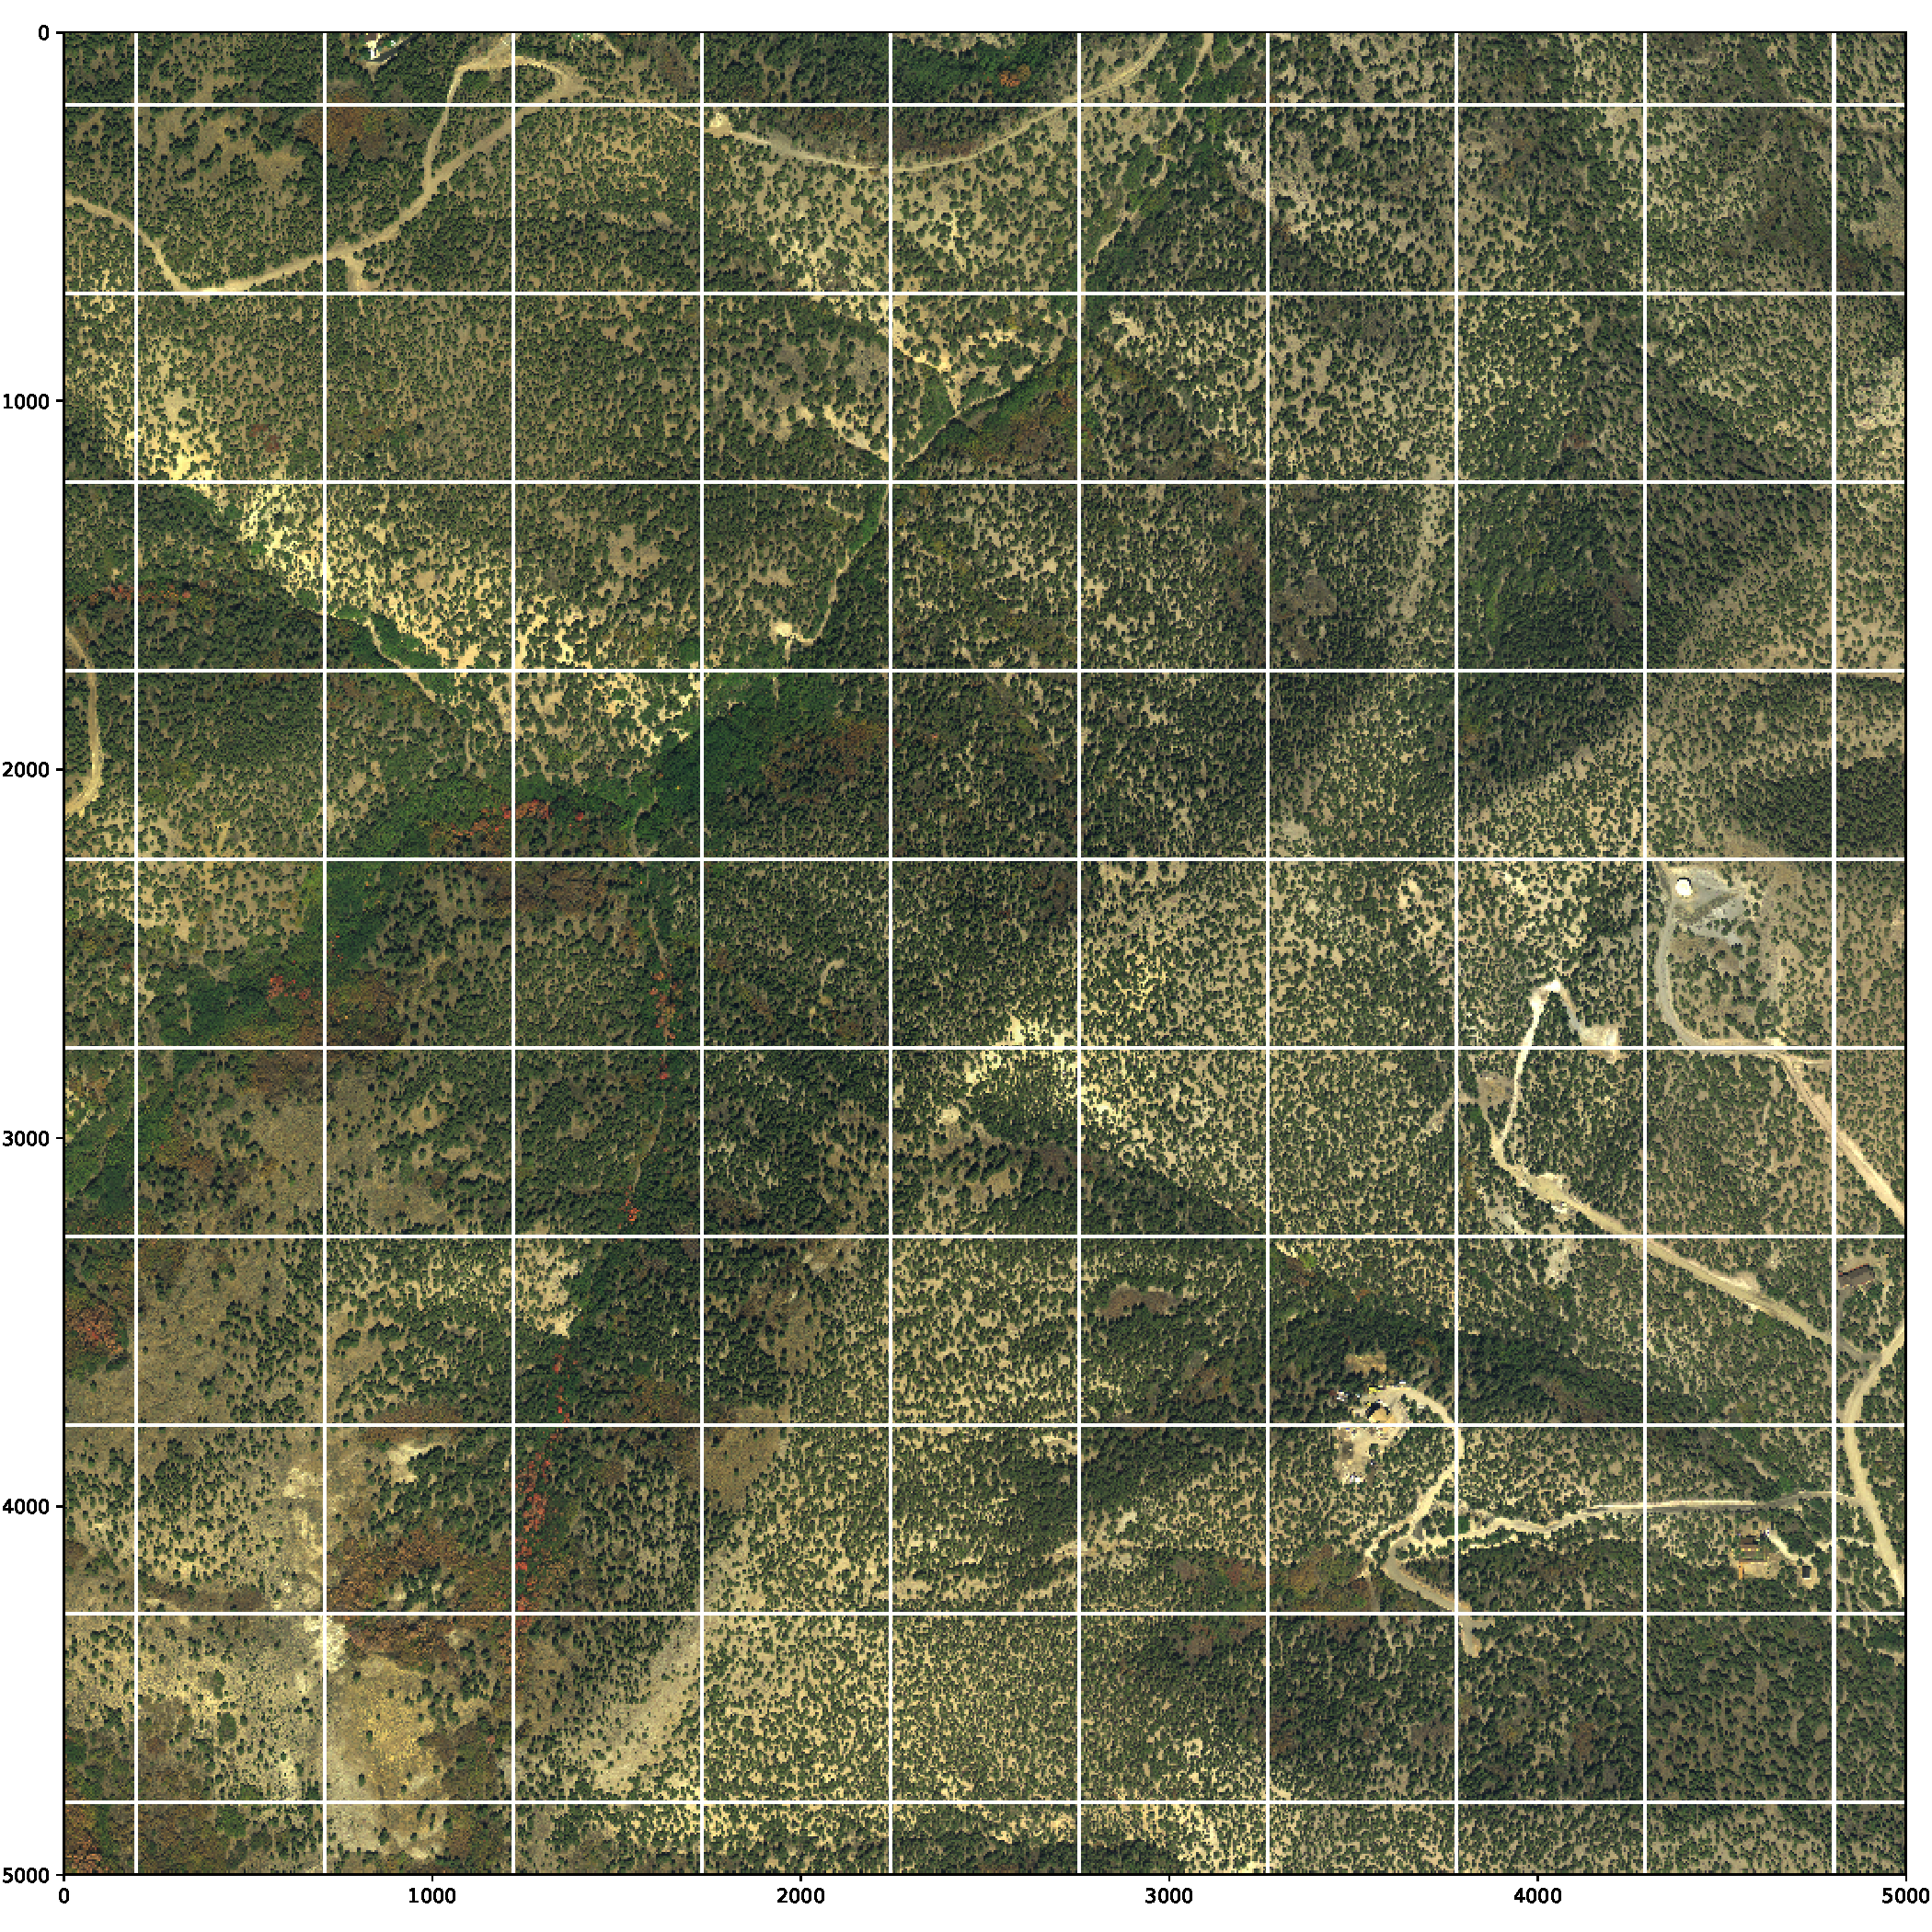
\includegraphics[width=1\textwidth]{Figures/example_unproc.pdf}
	\caption{\textbf{Example of unprocessed image.} This image has a size of $5000\times5000$ pixel. The continuous white lines are guidelines for the eye to demonstrate how we crop smaller images where we only return a cropped image from the white squares with size $512\times512$.}
	\label{fig:example-unproc}
\end{figure}

For the determination of relevant geographic locations we excluded cities and highly developed urban areas, and instead focussed on unpopulated areas. Specifically, we limited our image search to the four land use categories agriculture, shrubland-grassland, semi-desert, and forest-woodland that can be found in the USGS Land Cover Viewer. Note that these categories served as a rough geographic orientation to pin down geolocations of interest. However not all the images could be assigned with absolute certainty to one unique category since we were not able to overlay both maps. Further, we selected many images from national parks because we found that it is significantly harder to find imagery data that does not show human influence. Whenever possible we also tried to collect images from both classes (man-made vs. natural) within a given area/terrain.

\begin{figure}[h!]
	\centering
	\captionsetup{width=1\linewidth}
	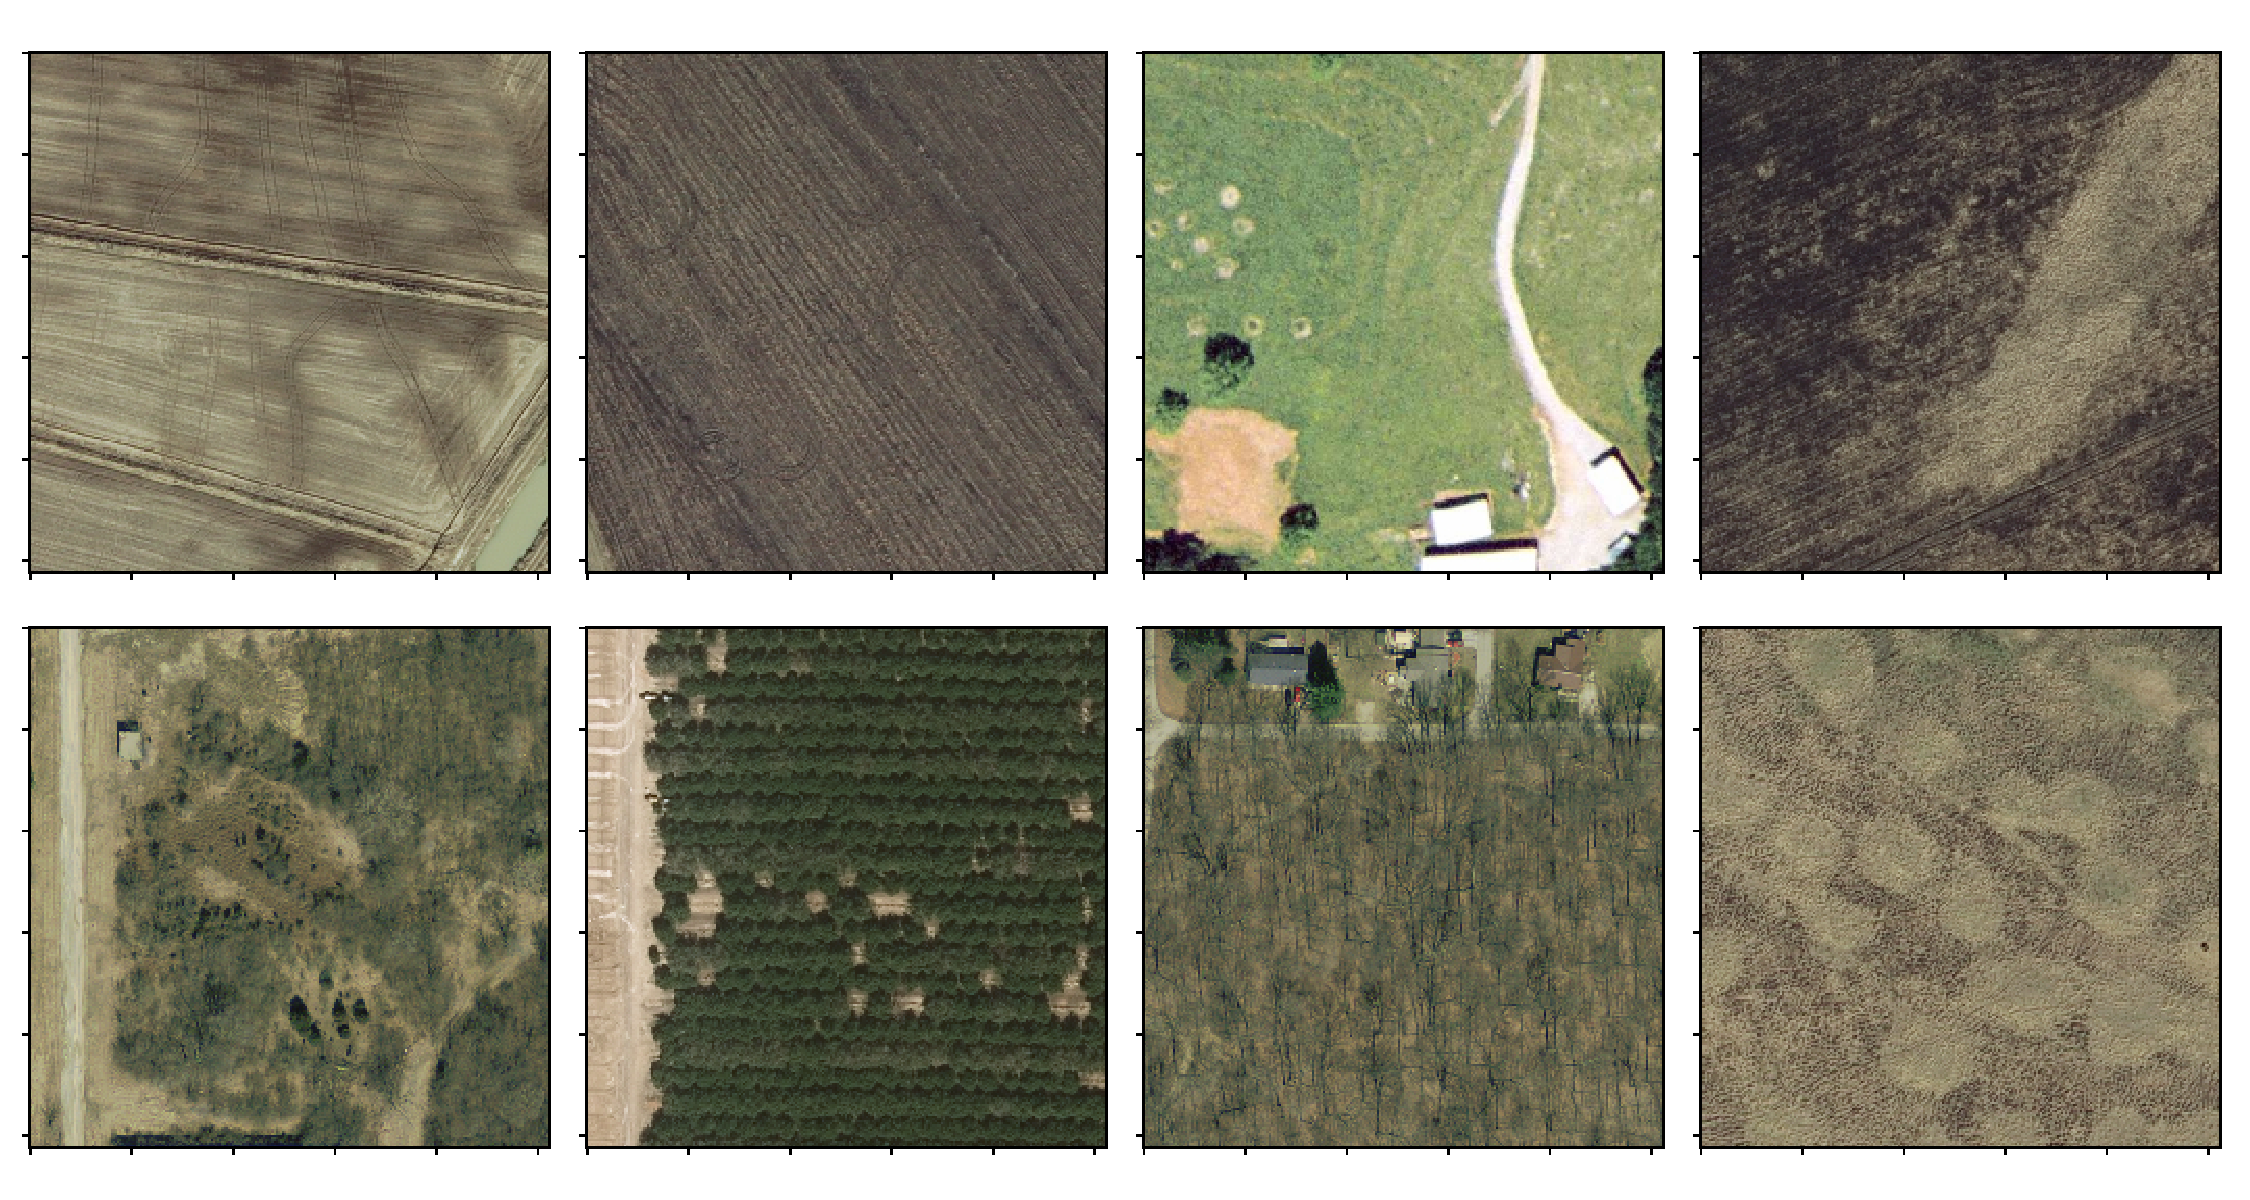
\includegraphics[width=1\textwidth]{Figures/agriculture_sample.pdf}
	\caption{\textbf{Example images of category Agricultue.} All images in this figure show clear signs of human impact. The images have a size of $512\times512$ pixels and a resolution of $0.3$m per pixel.}
	\label{fig:agriculture_sample}
\end{figure}

\begin{figure}[h!]
	\centering
	\captionsetup{width=1\linewidth}
	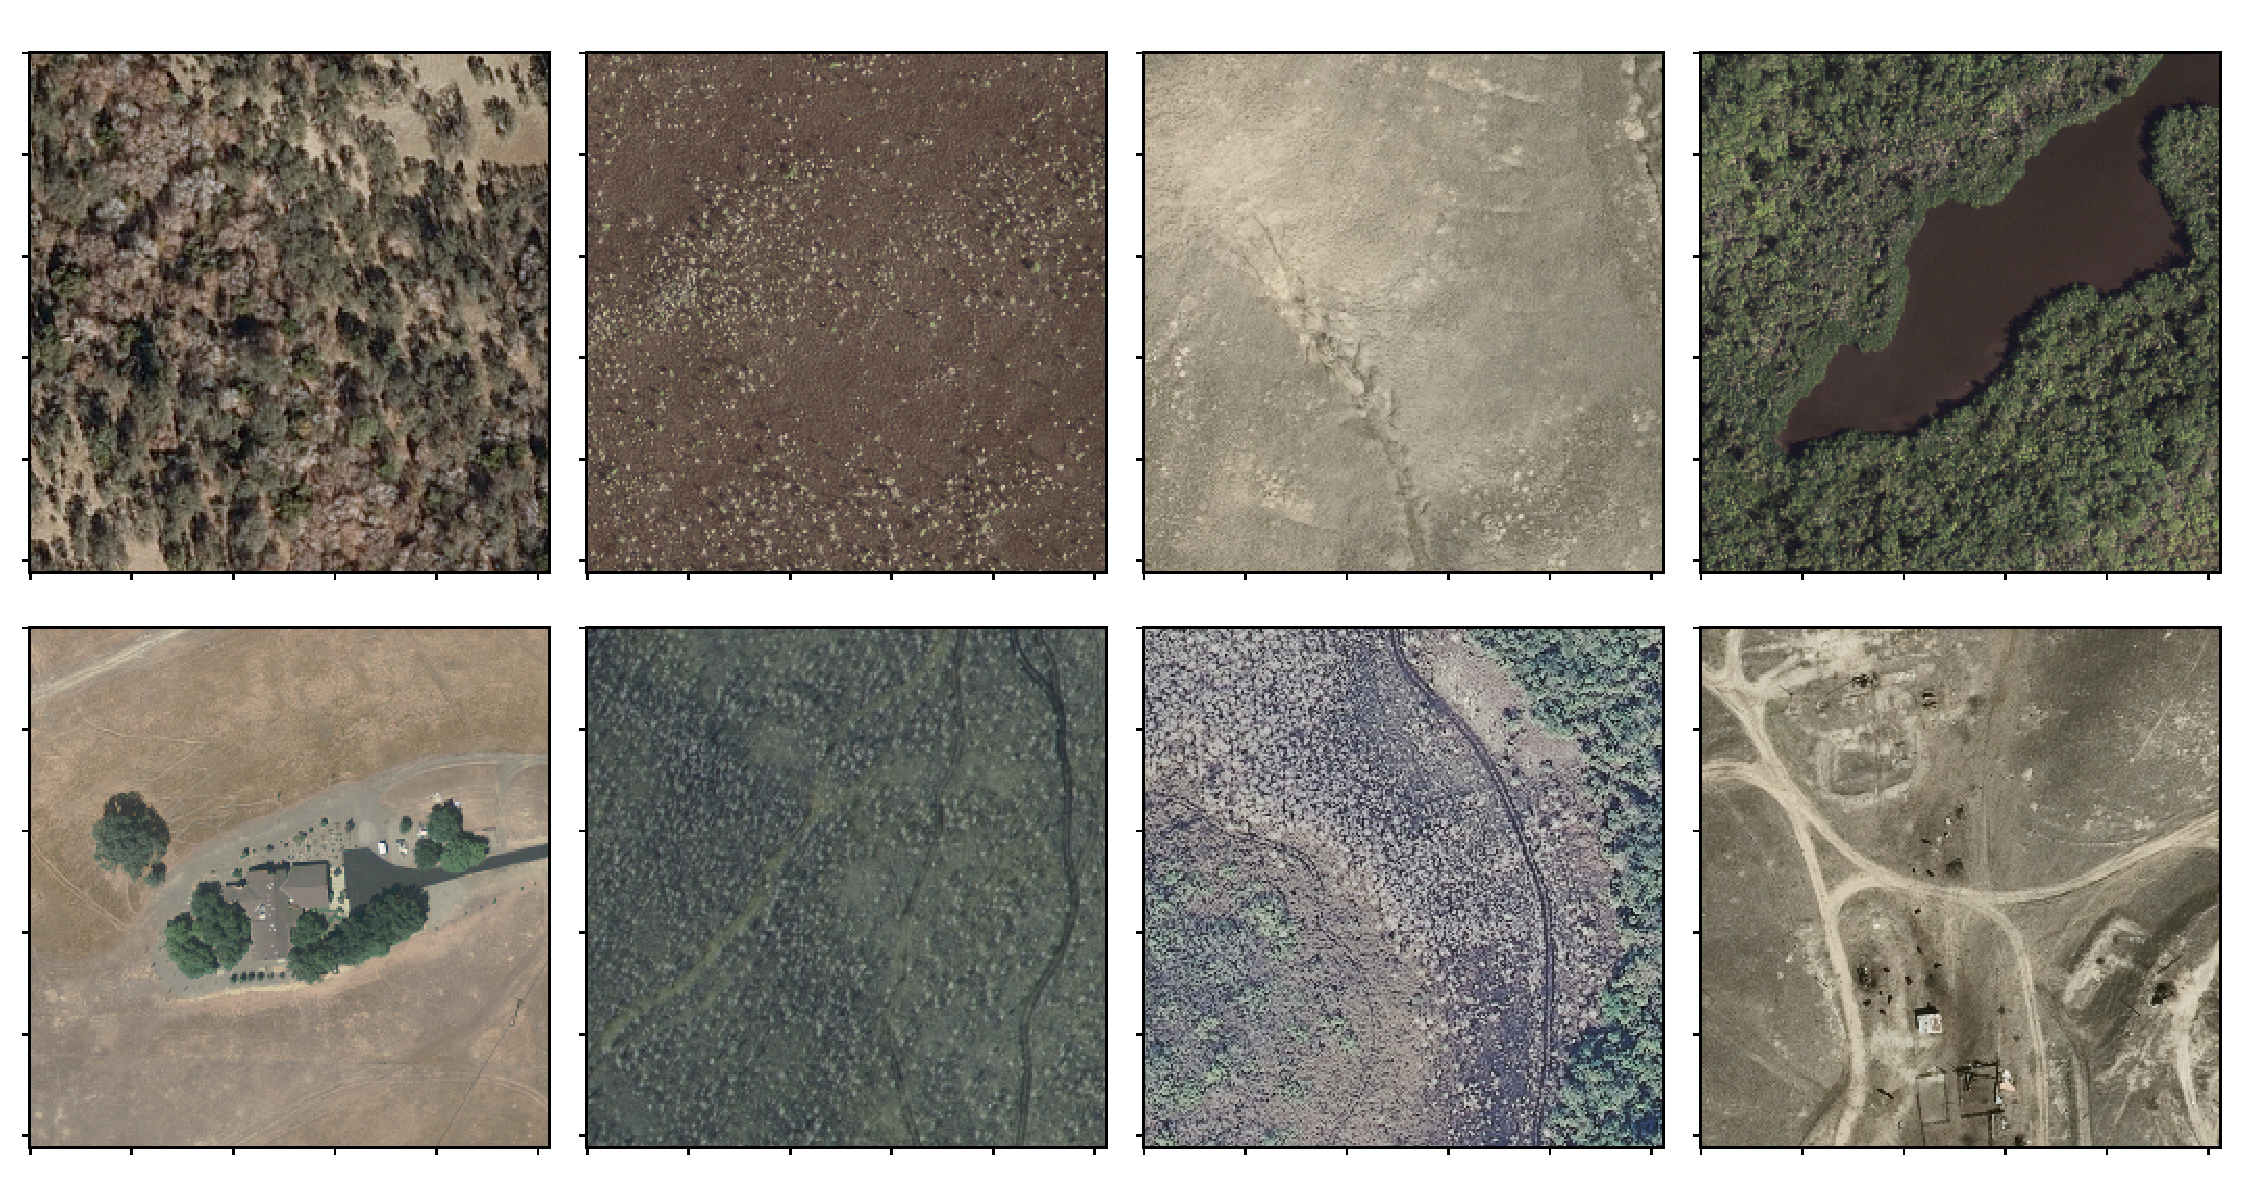
\includegraphics[width=1\textwidth]{Figures/shrubland-grassland_sample.pdf}
	\caption{\textbf{Example images of category shrubland-grassland.} The images in the first row do not contain any human influence, while the images in the second row show man-made structures. The images in this figure have a size of $512\times512$ pixels and a resolution of $0.3$m per pixel.}
	\label{fig:shrubland-sample}
\end{figure}

\begin{figure}[h!]
	\centering
	\captionsetup{width=1\linewidth}
	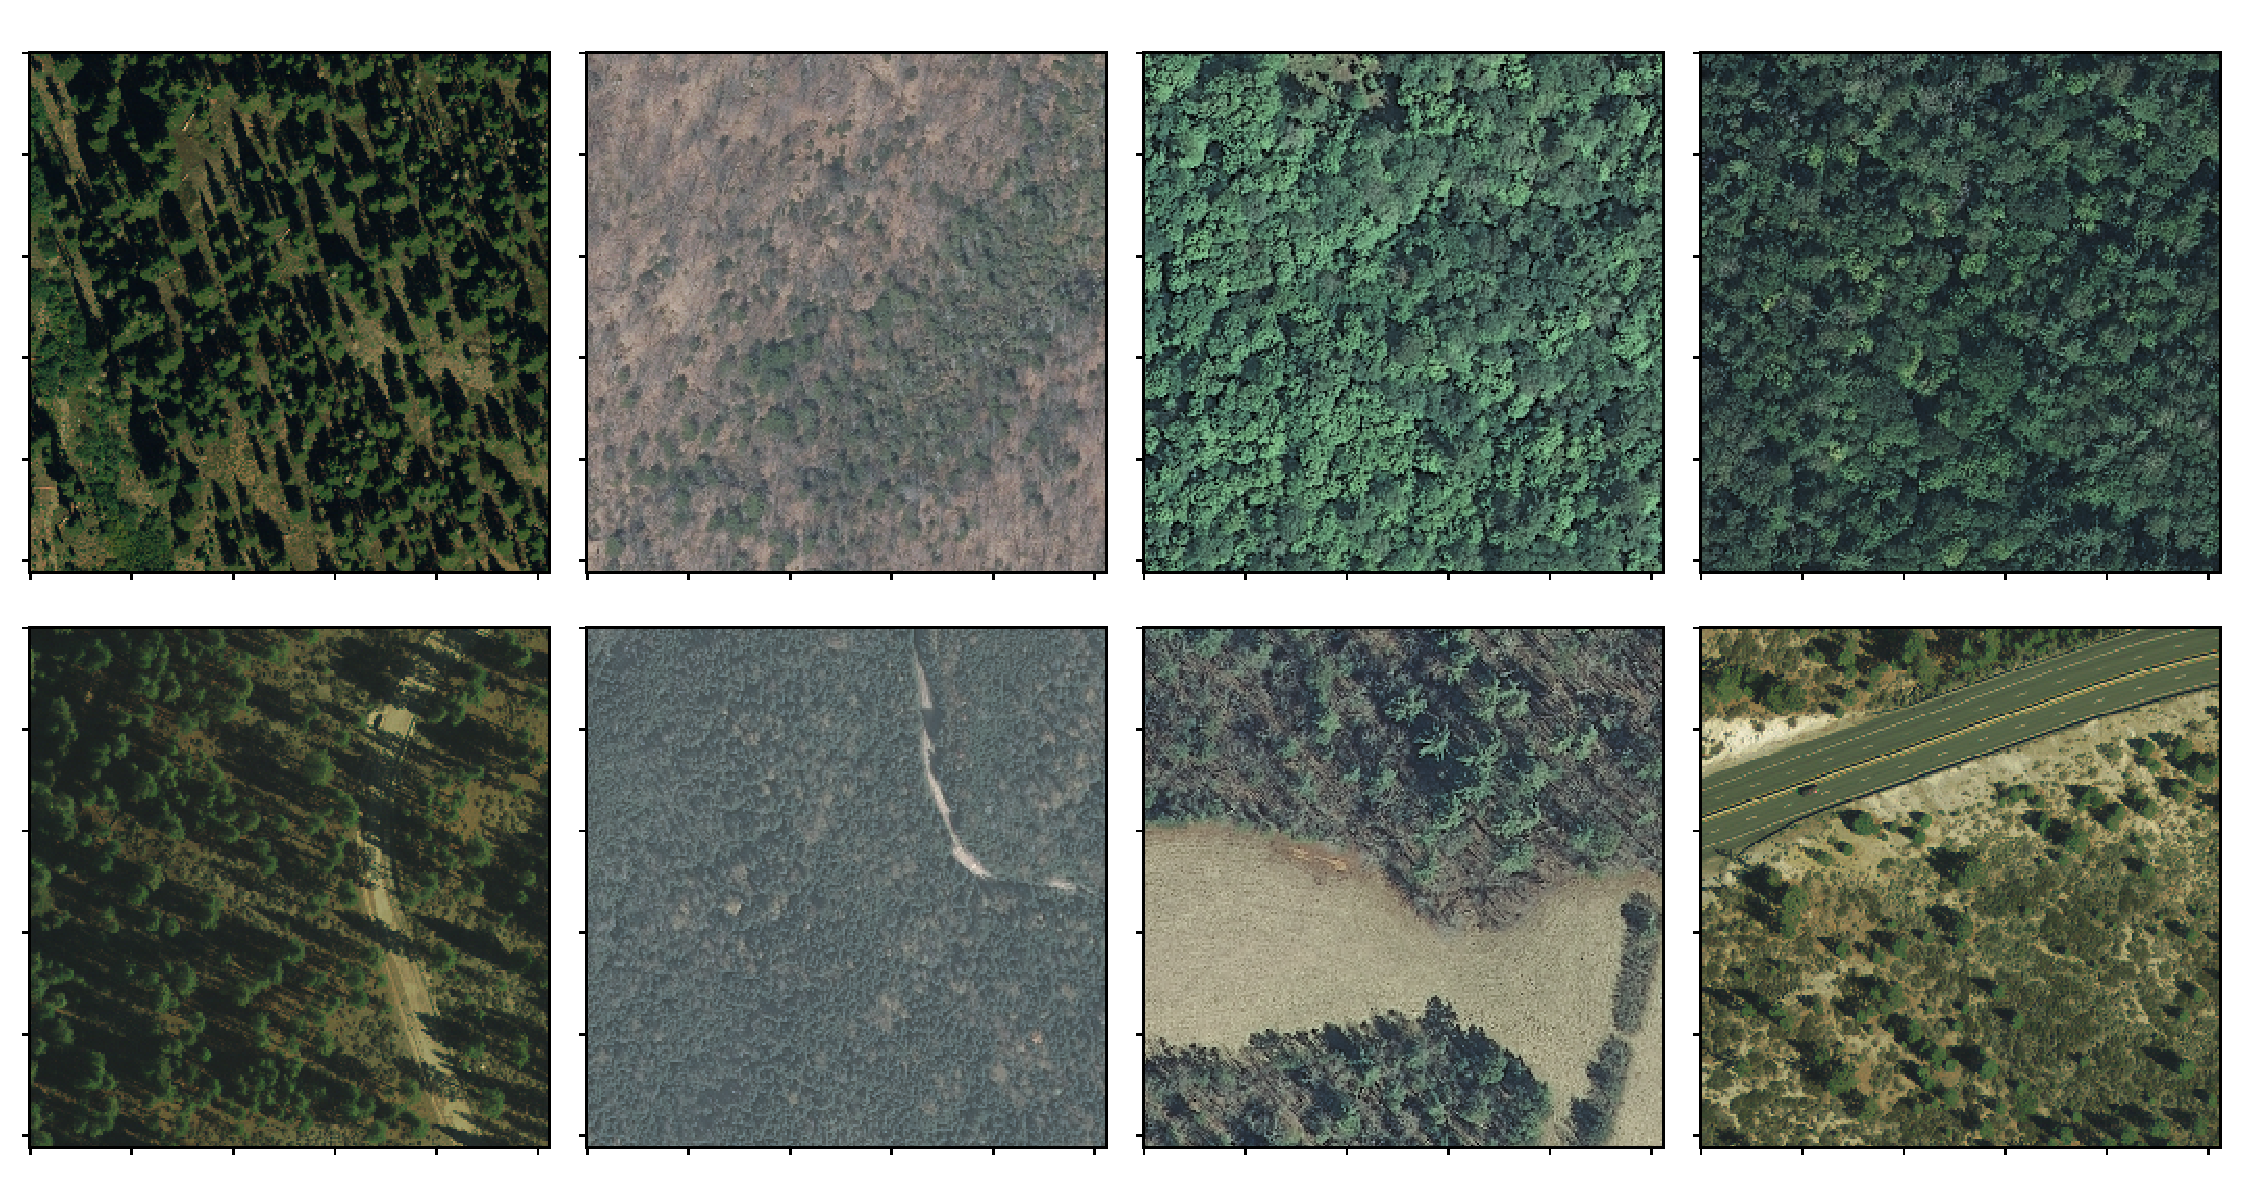
\includegraphics[width=1\textwidth]{Figures/forest-woodland_sample.pdf}
	\caption{\textbf{Example images of category forest-woodland.} The images in the first row do not contain any human influence, while the images in the second row show man-made structures. The images in this figure have a size of $512\times512$ pixels and a resolution of $0.3$m per pixel.}
	\label{fig:forest-sample}
\end{figure}

\begin{figure}[h!]
	\centering
	\captionsetup{width=1\linewidth}
	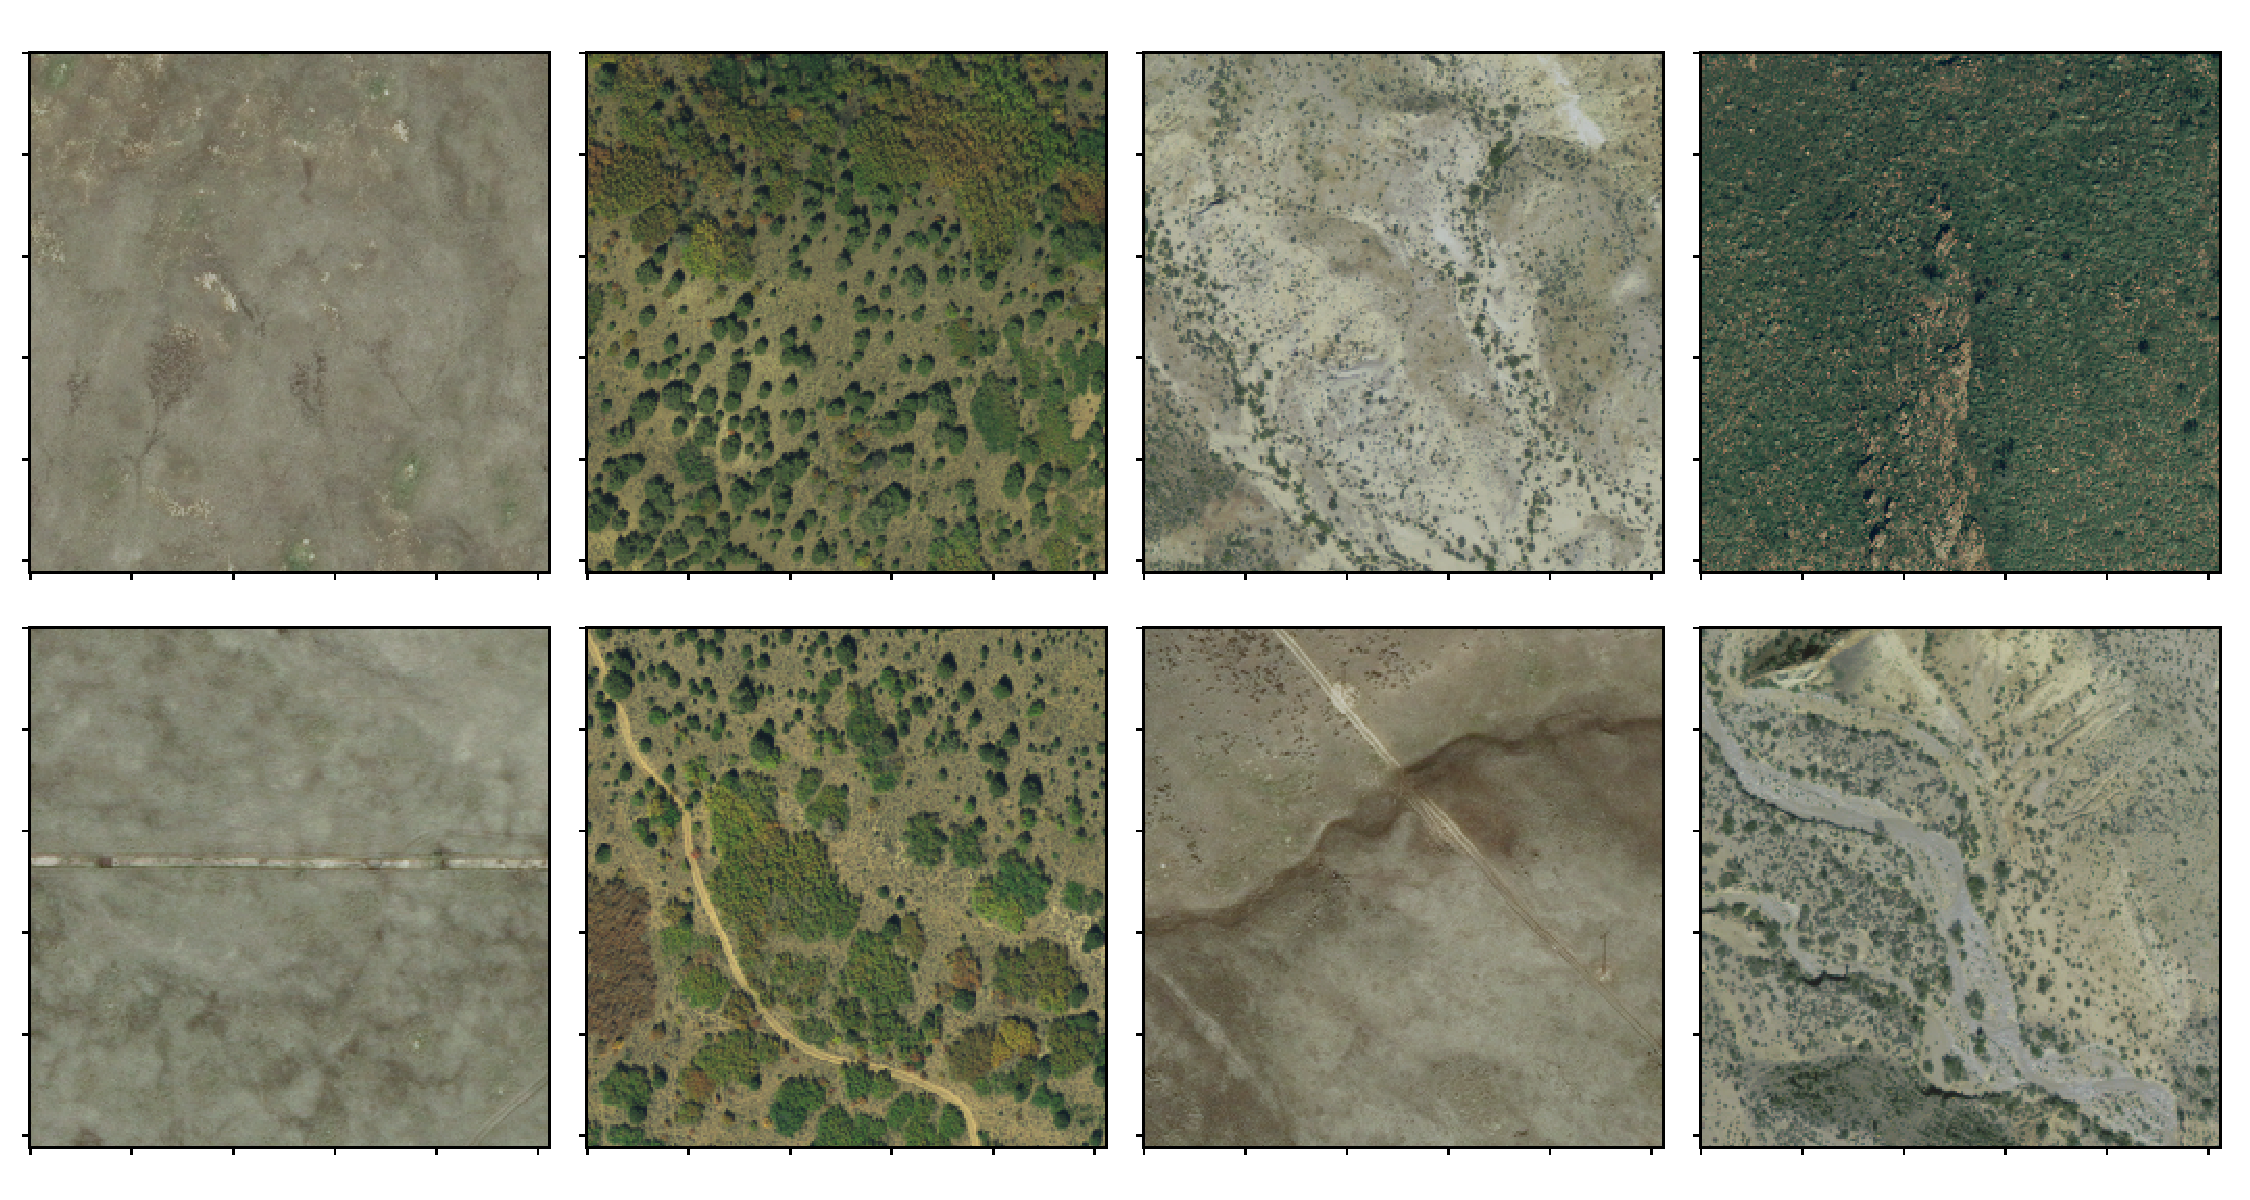
\includegraphics[width=1\textwidth]{Figures/semi-desert_sample.pdf}
	\caption{\textbf{Example images of category semi-desert.} The images in the first row do not contain any human influence, while the images in the second row show man-made structures. The images in this figure have a size of $512\times512$ pixels and a resolution of $0.3$m per pixel.}
	\label{fig:desert-sample}
\end{figure}

Once an area was pointed out as a region of interest, we located it on USGS Earthexplorer and downloaded images from that area. In particular, we constructed two datasets with 0.3m and 1m resolution, respectively. The former was taken from the category High Resolution Orthoimagery and the latter from the category National Agriculture Imagery Program (NAIP). Note that the images in these categories usually have a height and a width of several thousand pixels, and hence oocupy a few hundreds of Megabytes of disk space. We cropped smaller images out of the raw images, which will be discussed in more detail in the following section. Overall, we downloaded about 100 raw images for each dataset. An example is shown in Fig.~\ref{fig:example-unproc}.


\subsection{Data Processing and Labeling}
Our data processing pipeline consists of the following steps:
\begin{enumerate}
	\item Download large raw images.
	\item Crop images of size $512\times512$ pixel.
	\item Label images with either zero (no human impact), one (minimal human impact), two (clear human impact).
	\item Degrade images, i.e. reduce number of pixels and thereby resolution per pixel.
\end{enumerate}

Let us discuss each of these steps in more detail. An illustration of the first and second step of the image processing pipeline is given in Fig.~\ref{fig:example-unproc}. The white lines demonstrate the way we crop smaller images ($512\times512$) from the large raw image ($5000\times5000$). We process all raw images in this manner, which yields approximately 80-150 processed images per raw image. We hence obtain about 10,000 processed images for each dataset. Within each category (USGS Land Cover categories) of the processed images we labeled a selected portion of the images by moving them into the folder with the respective label name. 

We have published our datasets via a Google Drive link \parencite{datasets}. The image folder of the published datasets contains the raw images, the processed images, and the labeled images. In this folder we follow a specific folder structure, which is shown below. Here pointy brackets (<parameter>) indicate a parameter and the content in the optional curly braces determines whether it is a folder pertaining to raw images. The first parameter is $pixels = 512$ and the second parameter represents the resolution of the dataset. Note that the label folders only exist in the case of processed images.
\vspace{10px}
\dirtree{%
	.1 \{raw-images-\}usgs-<pixels>-res<resolution>m.
	.2 semi-desert.
	.3 label-0.
	.3 label-1.
	.3 label-2.
	.2 agriculture.
	.3 label-2.
	.2 shrubland-grassland.
	.3 label-0.
	.3 label-1.
	.3 label-2.
	.2 semi-desert.
	.3 label-0.
	.3 label-1.
	.3 label-2.
}
\vspace{10px}
Annotating the images with labels was performed following certain rules. First, we classified images with no human impact at all into the class with label zero,  while we classified images with very clear human influence into the class with label two. Ambigious images i.e. images with minimal human traces, such as a small walking path, were classified into class one. Second, we've put major effort into creating datasets that contain images of similar texture spread across all classes. If we for example classified a set of images of a certain forest type into class zero we classified another set of images with a similar forest type, but containing a building or a street, into the class two. We followed the latter rule for all categories except agriculture. The agriculture images all show human influence, and were therefore all classified with label two. By sticking to these rules, we are able to guarantee that the algorithm learns features that relate to the appearance of man-made structures, and not to image artefacts such as color or texture.

\begin{figure}[h!]
	\centering
	\captionsetup{width=1\linewidth}
	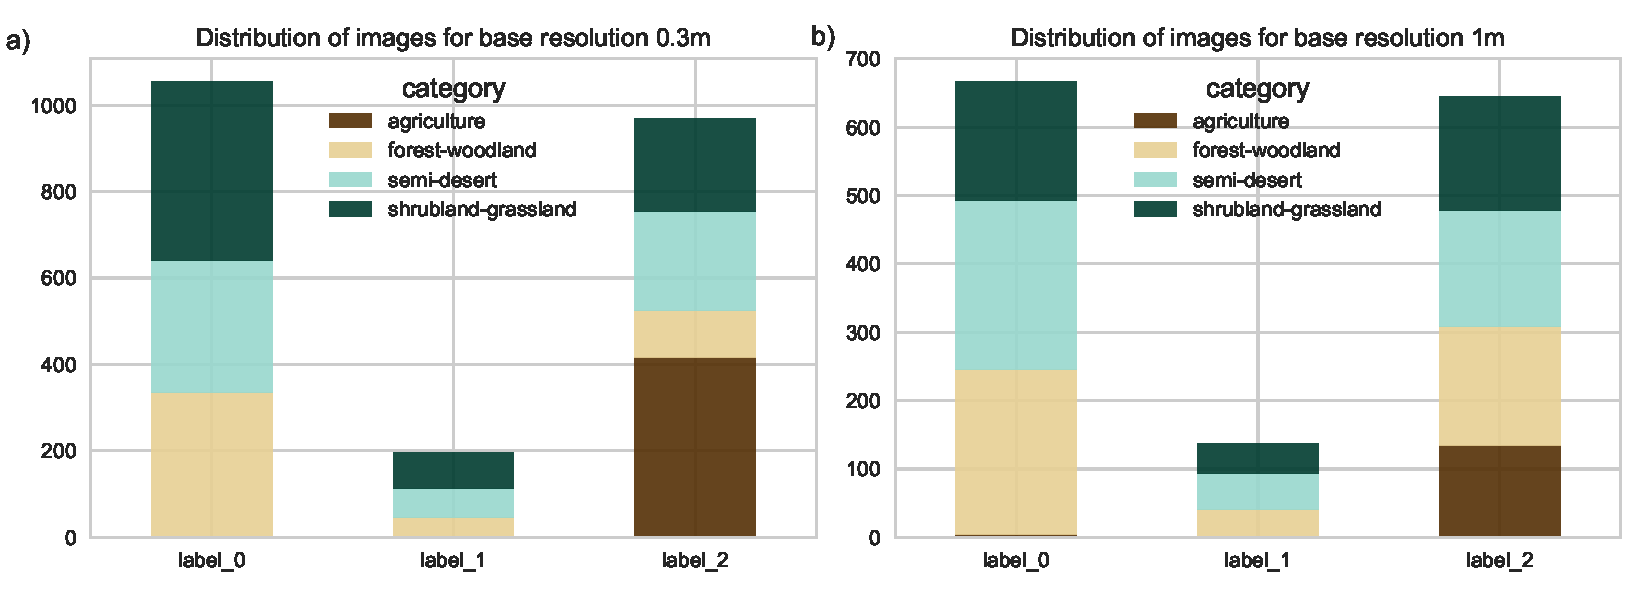
\includegraphics[width=1\textwidth]{Figures/imstats.pdf}
	\caption{\textbf{Number of images per category and label.} (a) Distribution of images for dataset with resolution of 0.3m per pixel. (b) Distribution of images for dataset with resolution of 1m per pixel.}
	\label{fig:imstats}
\end{figure}

In Figures \ref{fig:agriculture_sample} - \ref{fig:desert-sample} we display sample images for each of the four categories, repsectively. These images belong to the dataset that has a pixel resolution of 0.3m. The images from the 1m dataset have similar characteristics, but are not shown due to redundancy. Note that in Figs. \ref{fig:shrubland-sample} - \ref{fig:desert-sample} the first row represents images of label zero and the second row shows images that belong to label two. As mentioned above, the images in Fig.~\ref{fig:agriculture_sample} (agriculture) all contain human influence, and therefore belong to class two. 

The distribution of categories and labels is shown in Fig.~\ref{fig:imstats}. Overall, for the 0.3m dataset we classified about 2200 images, and for the 1m dataset we classified about 1450 images. Our main goal consisted in creating a balanced dataset between label zero and label two as can be seen from the distributions. A minority of images, roughly $10\%$ of all annotated images were assigned to label one. These images were used at random to investigate the behaviour of the Machine Learning classifier, which is discussed in chapter~\ref{Chapter4}.

\begin{figure}[h!]
	\centering
	\captionsetup{width=1\linewidth}
	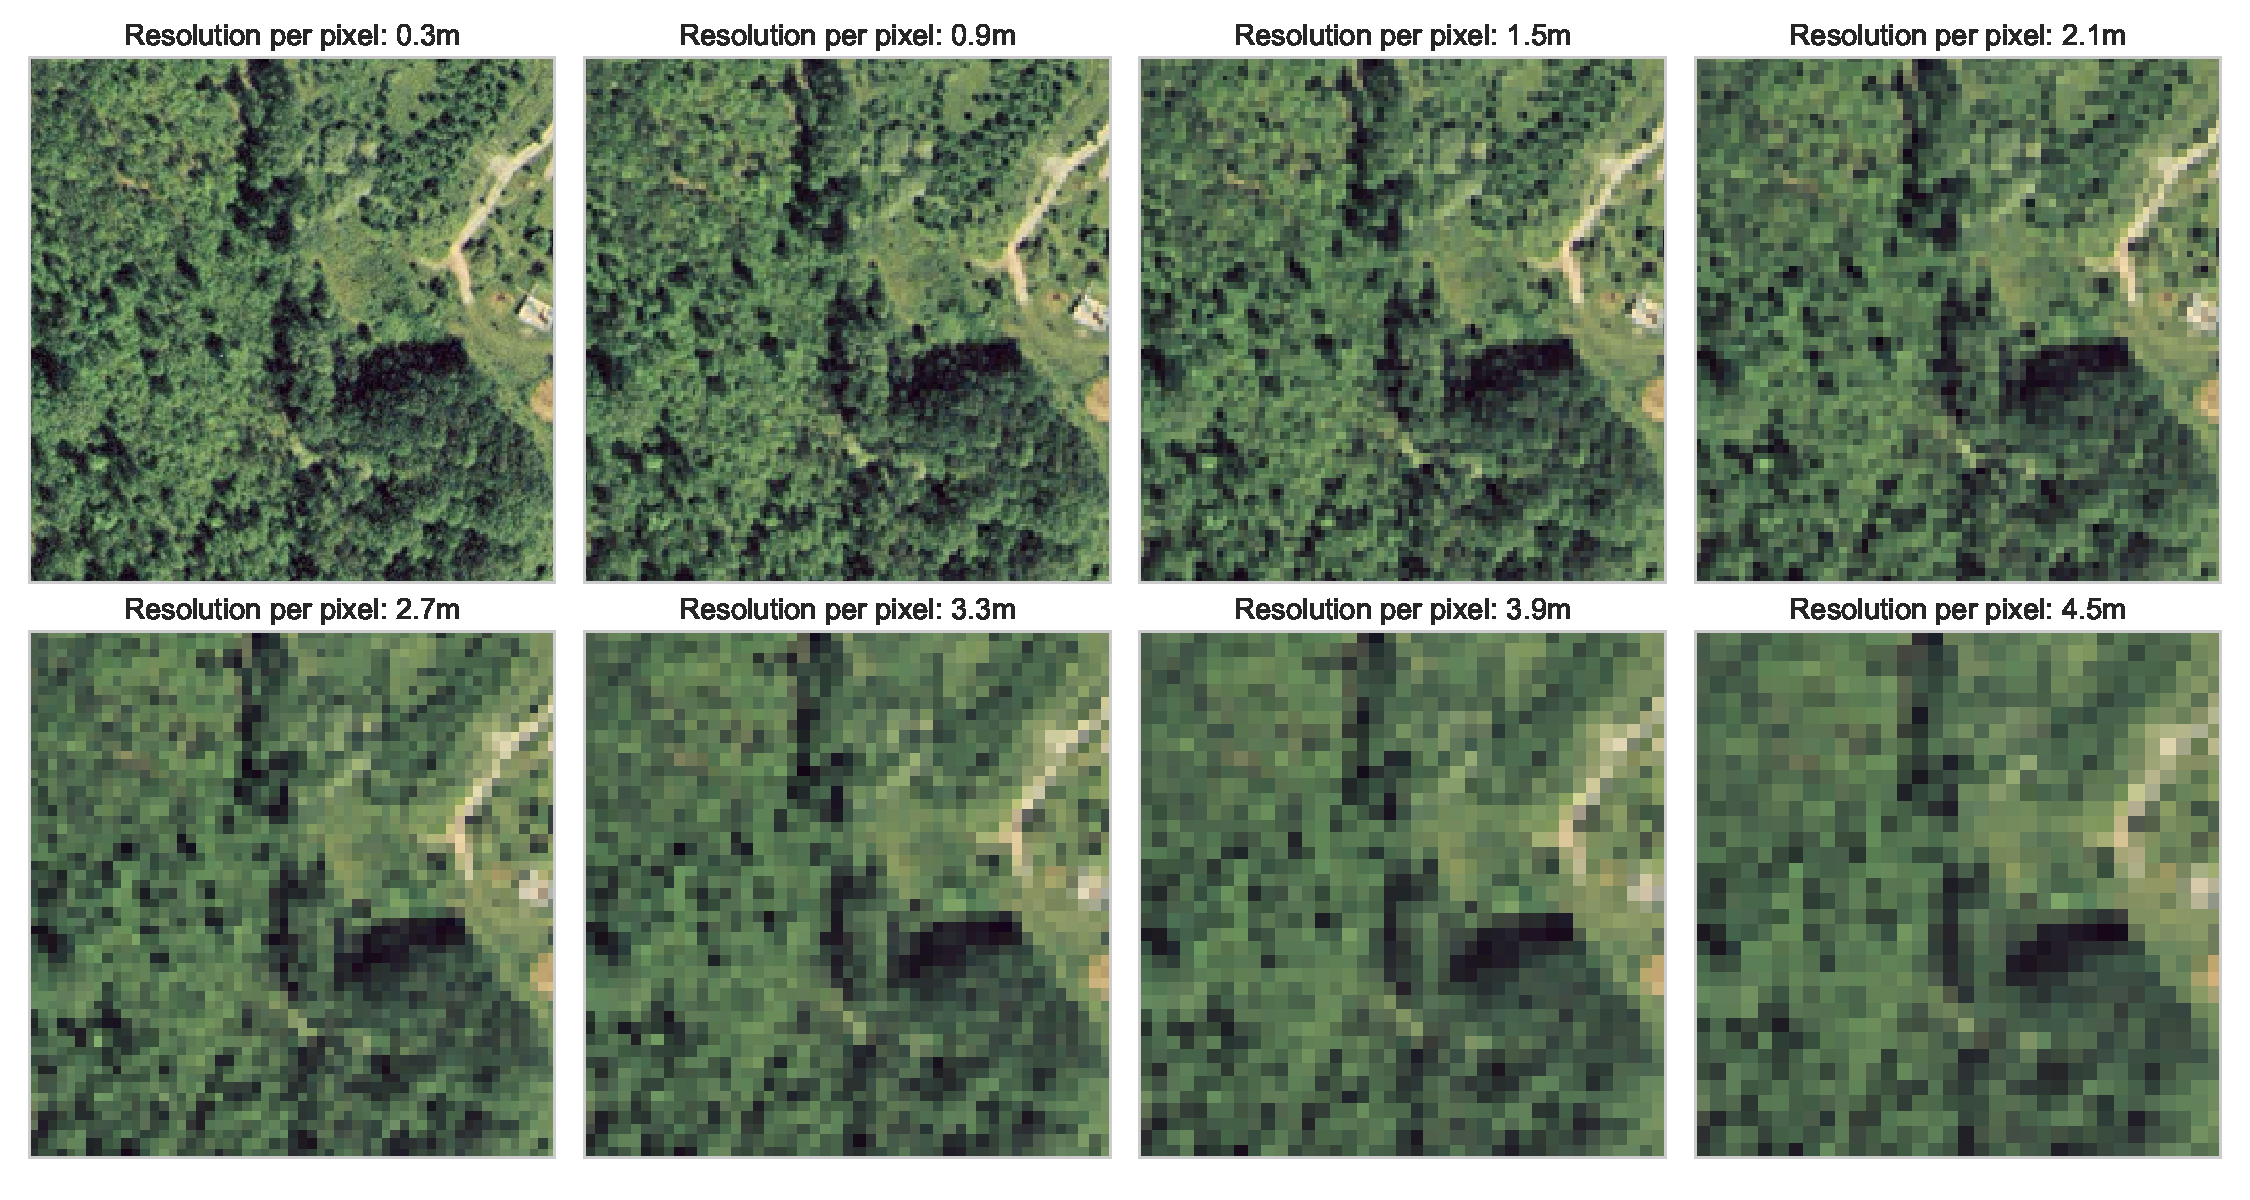
\includegraphics[width=1\textwidth]{Figures/demo_degrade.pdf}
	\caption{\textbf{Example of image downsampling}. The upper left image has a base resolution of 0.3m per pixel and a size of $512\times512$ pixels whereas the lower right image has the worst resolution, 4.5m per pixel, and a size of $34\times34$ pixels. All intermediate images are downsampled by a factor corresponding to the resolution of the actual image divided by the base resolution. For instance, for the lower right image the factor is 15.}
	\label{fig:degrade}
\end{figure}

The last step of the data processing pipeline consisted in downsampling the processed and labeled images, in order to obtain images with a lower resolution. We used a Lanczos filter \parencite{duchon1979} for the sampling, which is based on a sinusoidal kernel. In Fig.~\ref{fig:degrade} we show a few selected resolutions for an example image from the agriculture category. Note that here we only schematically depict an example in order to illustrate the process. However, in our Machine Learning pipeline the images are downsampled on the fly and the result of this process is not stored on disk (see Section \ref{sec:dl_architecture} for further details).

For this particular image one can observe how certain image features disappear as the image quality is decreased. Above a resolution of around 3m per pixel one is not able anymore to identify the building close to the right corner of the image. 
The texture of the track that leads up to the building is blurred above a resolution of around 4m per pixel. This shows how different elements in an image are not recognizable anymore once the resolution approaches their characteristic size.



%----------------------------------------------------------------------------------------


\chapter{Neural Networks} 

\label{Chapter2}

%----------------------------------------------------------------------------------------
%	SECTION 1
%----------------------------------------------------------------------------------------

\section{Neural Networks}

Lorem ipsum dolor sit amet, consectetur adipiscing elit. Aliquam ultricies lacinia euismod. Nam tempus risus in dolor rhoncus in interdum enim tincidunt. Donec vel nunc neque. In condimentum ullamcorper quam non consequat. Fusce sagittis tempor feugiat. Fusce magna erat, molestie eu convallis ut, tempus sed arcu. Quisque molestie, ante a tincidunt ullamcorper, sapien enim dignissim lacus, in semper nibh erat lobortis purus. Integer dapibus ligula ac risus convallis pellentesque.

%-----------------------------------
%	SUBSECTION 1
%-----------------------------------

\subsection{Subsection 1}

Nunc posuere quam at lectus tristique eu ultrices augue venenatis. Vestibulum ante ipsum primis in faucibus orci luctus et ultrices posuere cubilia Curae; Aliquam erat volutpat. Vivamus sodales tortor eget quam adipiscing in vulputate ante ullamcorper. Sed eros ante, lacinia et sollicitudin et, aliquam sit amet augue. In hac habitasse platea dictumst.

%----------------------------------------------------------------------------------------
%	SECTION 2
%----------------------------------------------------------------------------------------

\section{Convolutional Neural Networks}

Sed ullamcorper quam eu nisl interdum at interdum enim egestas. Aliquam placerat justo sed lectus lobortis ut porta nisl porttitor. Vestibulum mi dolor, lacinia molestie gravida at, tempus vitae ligula. Donec eget quam sapien, in viverra eros. Donec pellentesque justo a massa fringilla non vestibulum metus vestibulum. Vestibulum in orci quis felis tempor lacinia. Vivamus ornare ultrices facilisis. Ut hendrerit volutpat vulputate. Morbi condimentum venenatis augue, id porta ipsum vulputate in. Curabitur luctus tempus justo. Vestibulum risus lectus, adipiscing nec condimentum quis, condimentum nec nisl. Aliquam dictum sagittis velit sed iaculis. Morbi tristique augue sit amet nulla pulvinar id facilisis ligula mollis. Nam elit libero, tincidunt ut aliquam at, molestie in quam. Aenean rhoncus vehicula hendrerit. 

\chapter{Deep Learning Approach}

\label{Chapter4}

%----------------------------------------------------------------------------------------

In the previous chapters we have introduced the key components of the approach we followed in our study: on the one hand, we have described existing satellite image datasets and introduced the actual data we will consider, and on the other, we have discussed Deep Learning, how it works and how we can use it for our problem. Now, we are ready to describe our approach: the image feature extraction, the model architecture and the training scenario.

\section{Image features and transfer learning}\label{sec:transferLearning}

In order to train a model based on images, some sort of features need to be extracted. Traditionally, this image feature extraction was based on a set of hand-crafted detectors aimed to detect edges, corners, blobs and other feature descriptors. Some of these detectors are the Sobel filter, Laplacian of Gaussian (LoG), Difference of Gaussians (DoG), Determinant of Hessian (DoH), SIFT \parencite{Lowe1999,Lowe2004}, SURF \parencite{Bay2006}, Histograms of Oriented Gradients (HOG) \parencite{Dalal2005} and Gabor filters.

\begin{figure}[h!]
	\centering
	\begin{subfigure}{.5\textwidth}
  		\centering
  		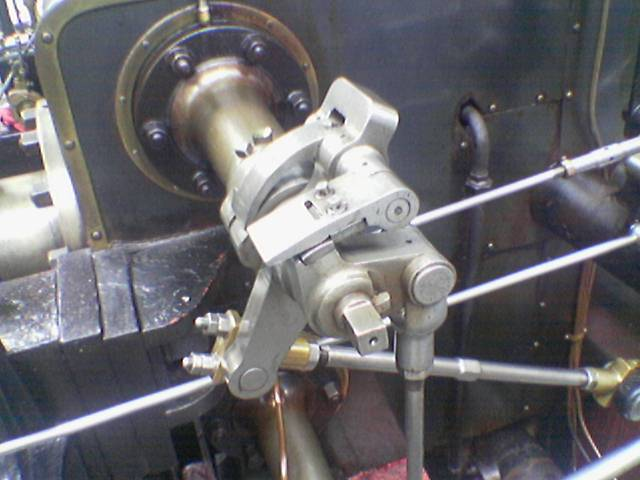
\includegraphics[width=.9\linewidth]{sobel_valve_original.png}
	\end{subfigure}%
	\begin{subfigure}{.5\textwidth}
  		\centering
  		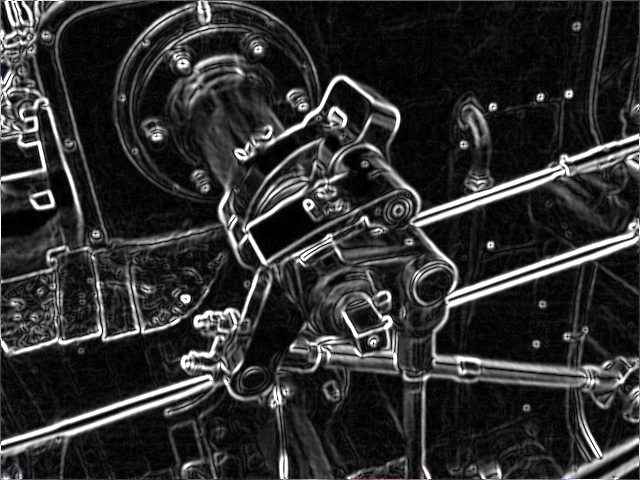
\includegraphics[width=.9\linewidth]{sobel_valve_processed.png}
	\end{subfigure}
	\captionsetup{width=1\linewidth}
	\caption{\textbf{Example of the Sobel filter}}
	\label{fig:sobel}
\end{figure}

\begin{figure}[h!]
	\centering
	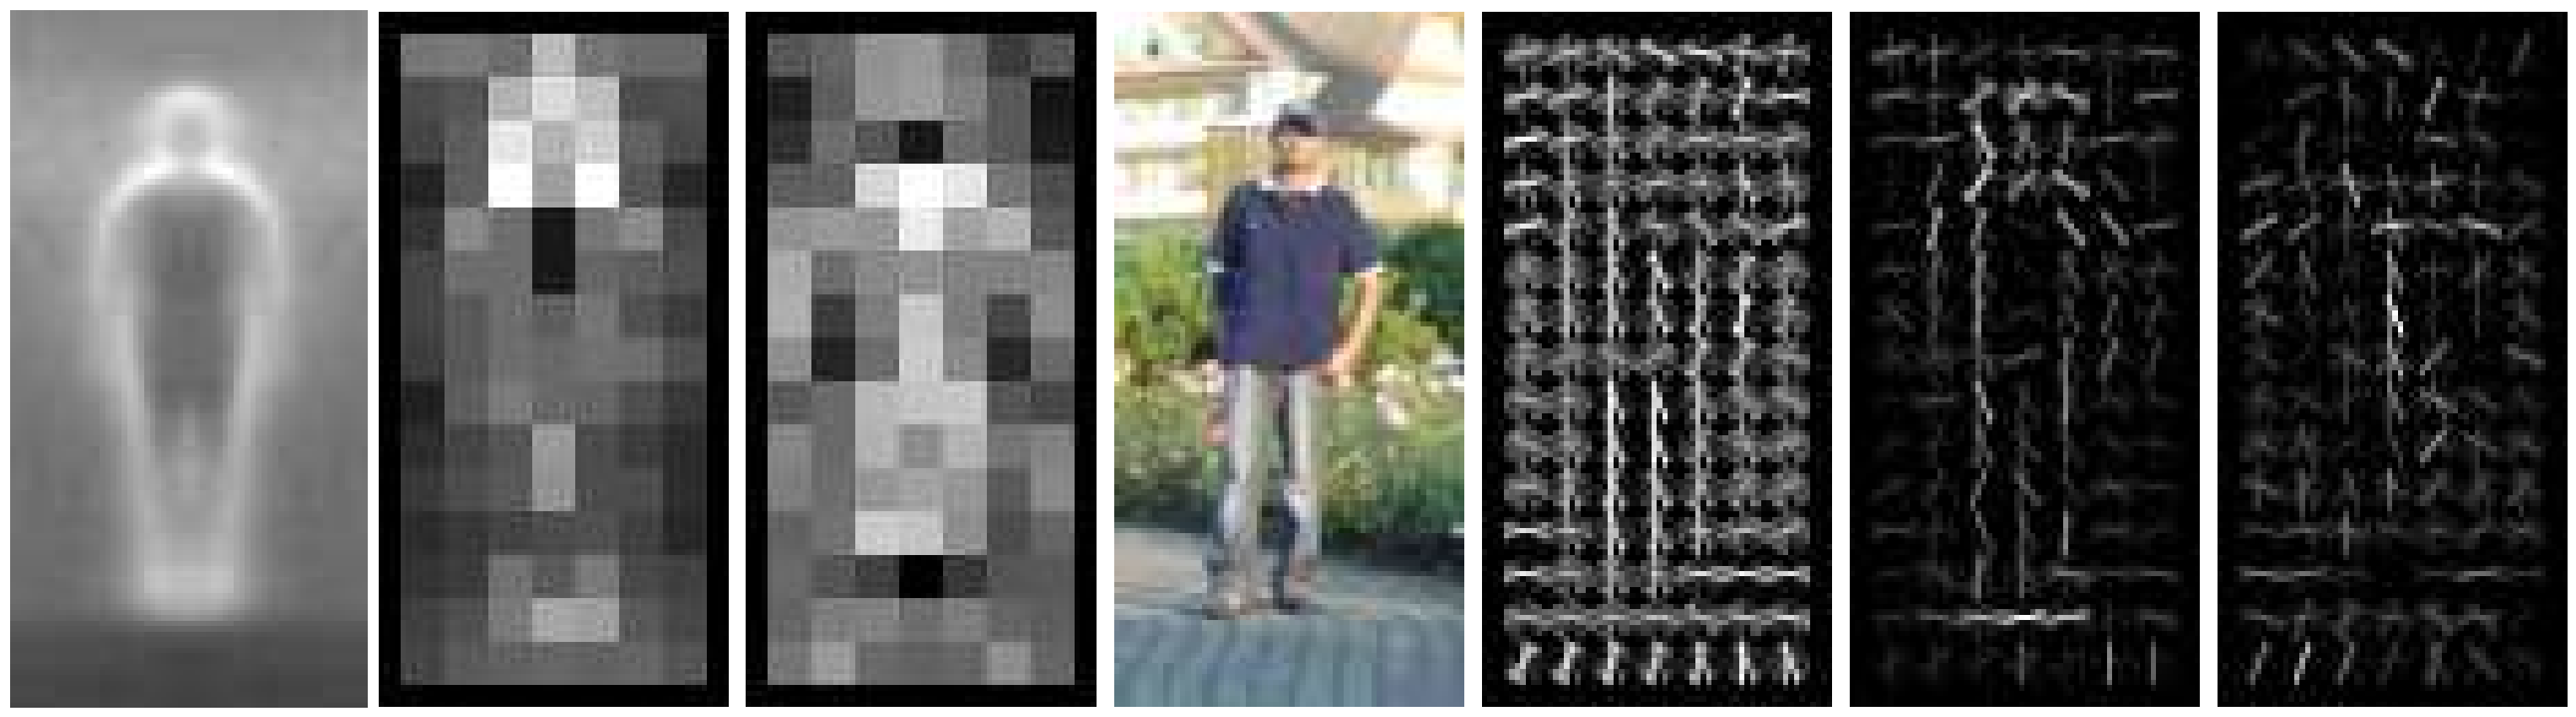
\includegraphics[width=0.9\textwidth]{Figures/hog_example.png}
	\captionsetup{width=1\linewidth}
	\caption{\textbf{Examples of HOG detector \parencite{Dalal2005}}}
	\label{fig:hog}
\end{figure}

More recent approaches to image classification using Neural Networks have benefited from the existing and increasing computational power, and deep Convolutional Neural Networks have been able to achieve higher performances than traditional models. 

Yet, training a deep CNN from scratch for a particular problem requires a large and exhaustive dataset along with a huge amount of computational power. However, it has been shown that the architectures of pre-trained NN can be reused for other purposes and achieve an equally great performance. This is known as \textbf{Transfer Learning}. Figure \ref{fig:transfer_learning_idea} schematizes this idea.

\begin{figure}[h!]
	\centering
	\captionsetup{width=1\linewidth}
	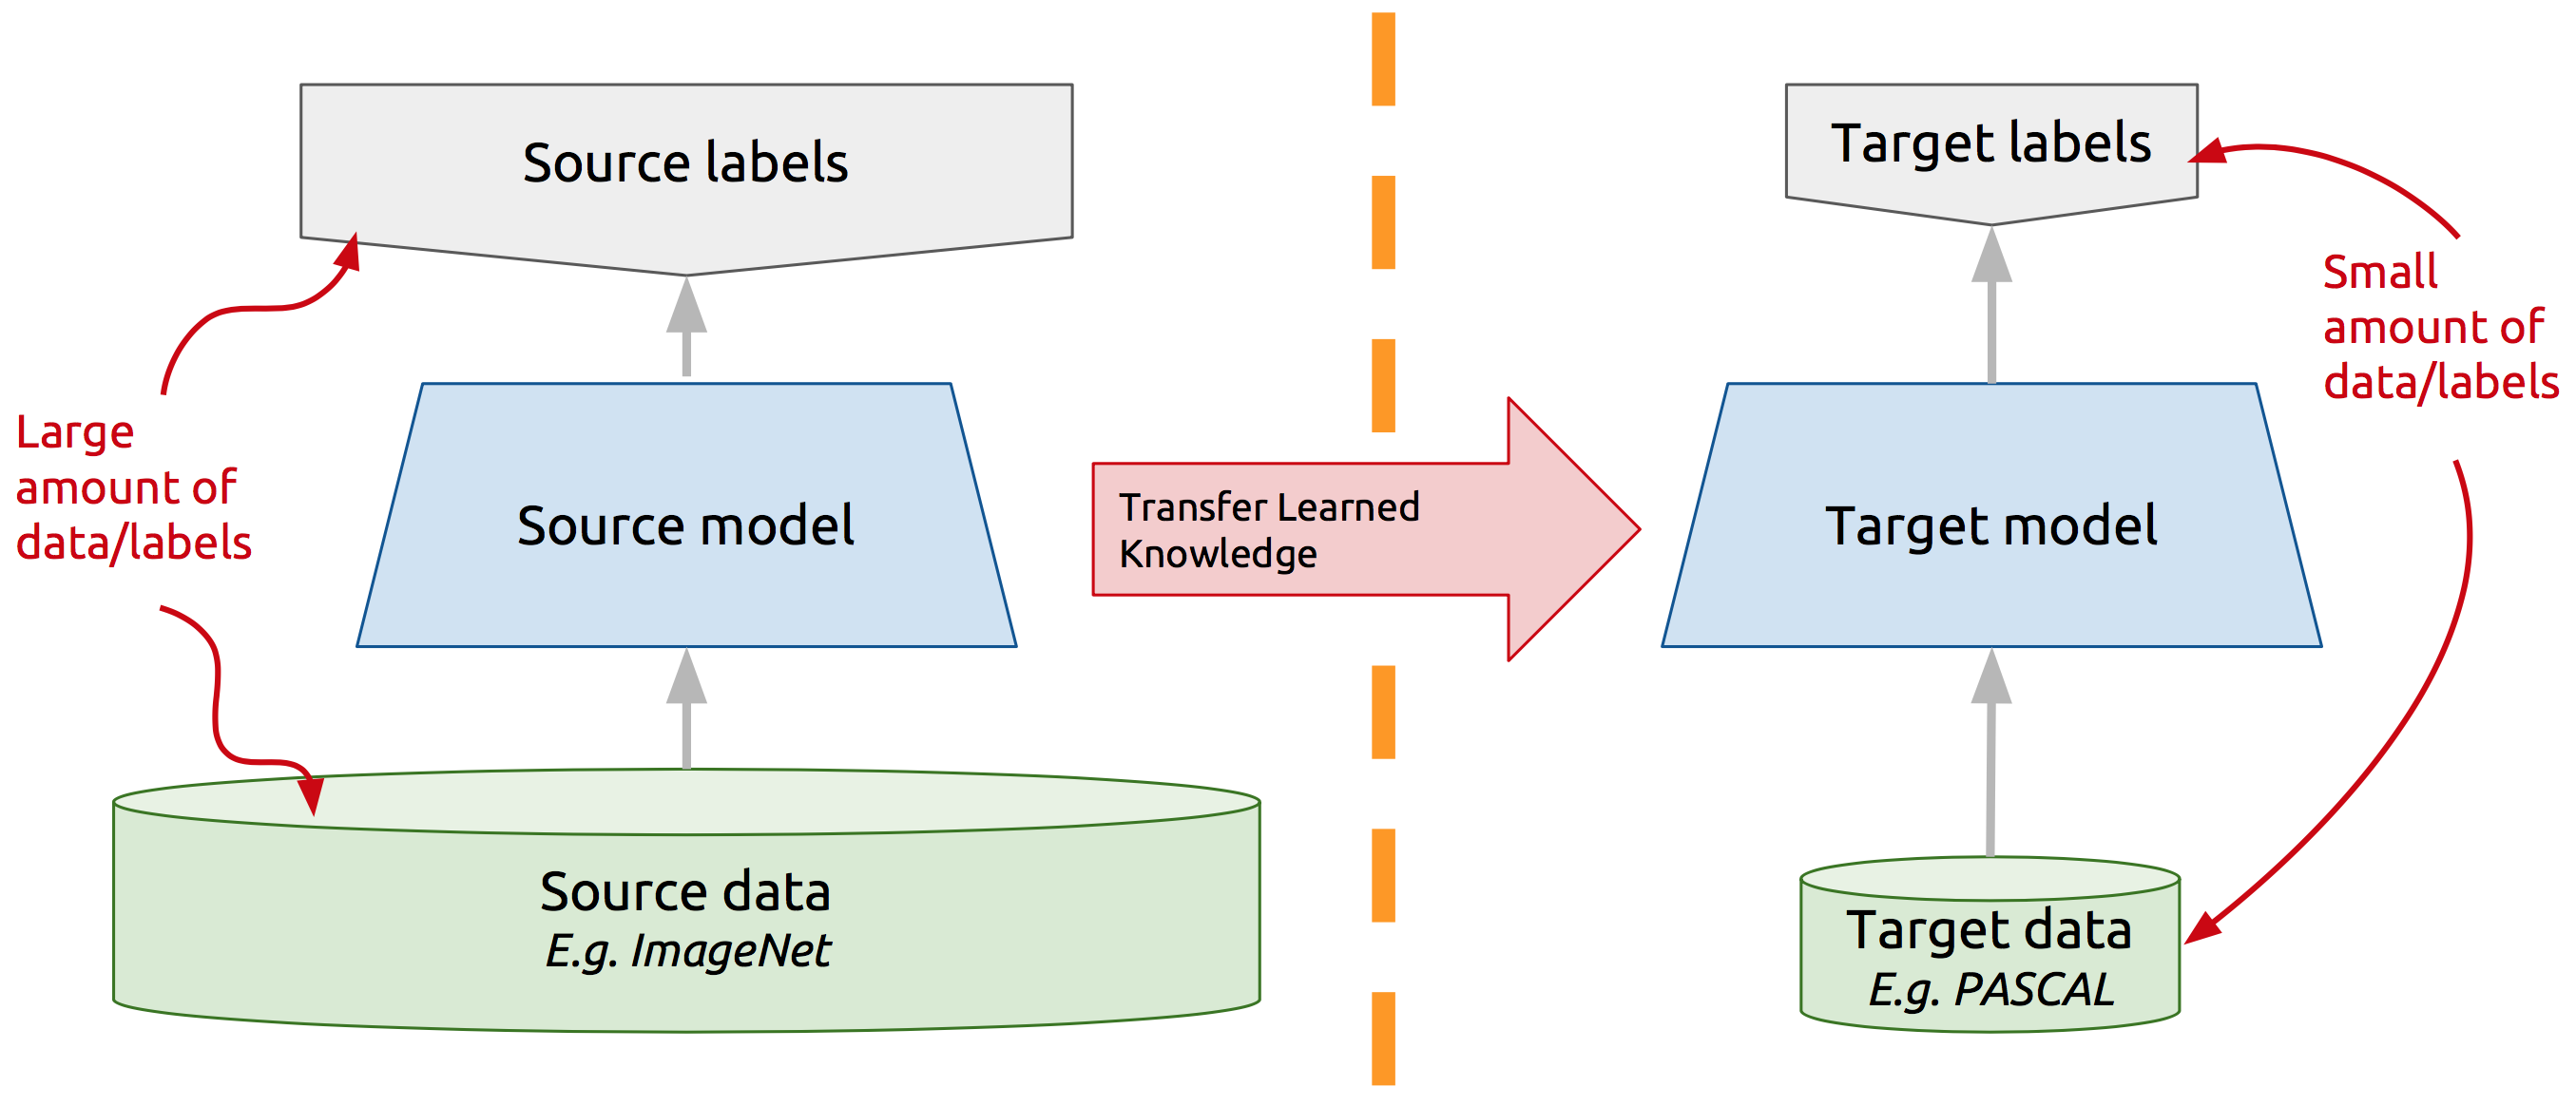
\includegraphics[width=1\textwidth]{Figures/transfer_learning_idea.png}
	\caption{\textbf{Transfer Learning}: a model learned from a large dataset can be transferred and reused for another purpose. \parencite{McGuinness2017}}
	\label{fig:transfer_learning_idea}
\end{figure}

These pre-trained architectures can be re-purposed by reusing the learned weights and either replacing the final layers of the net by some other classifier, or even fine-tuning all the layers for the specific problem. In any case, the initial layers of the Neural Network provide a great image feature extractor.

\

In the next section we describe our approach using transfer learning from a ResNet architecture.

%Consequently, there is an increasing library of available pre-trained models and weights: Xception, VGG, InceptionV3, ResNet.
%Most of these models have weights pre-trained on ImageNet, a large dataset containing more than 14 million hand-annotated images and over 20.000 categories.

%\begin{figure}[h!]
%	\centering
%	\captionsetup{width=1\linewidth}
%	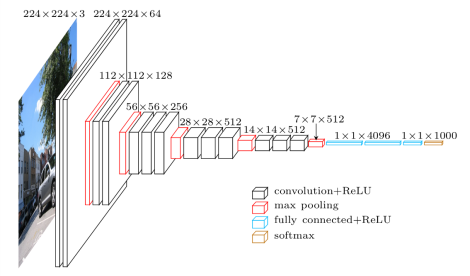
\includegraphics[width=1\textwidth]{Figures/imagenet_vgg16.png}
%	\caption{\textbf{VGG16 architecture}. Stack of $3\times 3$ convolutional and max pooling layers.}
%	\label{fig:degrade}
%\end{figure}

%\subsection{ResNets}

%Experience with Neural Networks, and CNN in particular, show that deeper nets tend to perform better, as these are more capable to model higher complexity. Yet, at some depth point, training becomes too difficult, because the gradient values obtained from the loss function are lost after several layers. This is known as \textbf{vanishing gradient}. ResNet fixes this is issue with Residual...

\section{Proposed architecture}\label{sec:dl_architecture}

As described before (Sections \ref{sec:CNNArchitectures} and \ref{sec:transferLearning}), we can use for our problem a pre-trained ResNet with our own final classification layers. Hence, the architecture we propose for our problem consists on the activation layers of a ResNet, which act as the feature extractors of our images, followed by a shallow classifier made of a single Dense (Fully Connected) layer. Figure \ref{fig:transfer_learning} gives a schema of this approach.

\begin{figure}[h!]
	\centering
	\captionsetup{width=1\linewidth}
	\includegraphics[width=1\textwidth]{Figures/transfer_learning.png}
	\caption{\textbf{Transfer Learning from a ResNet} (figure adapted from \parencite{McGuinness2017})}
	\label{fig:transfer_learning}
\end{figure}

\subsection{ResNet activations}

The ResNet we consider (ResNet50) has a total of $49$ activation layers, so the output at each of them is different. Initial layers are able to recognize edges, textures and patterns while keeping and image size similar to the input. On the other hand, deeper activation layers show more convoluted relations and provide much more channels (or filters) by shrinking the image size.

For instance, for an input image of (tensor) size $512 \times 512 \times 3$ (a $512x512$ image with $3$ RGB channels), the output of the first activation layer is of size $256 \times 256 \times 64$, the $10^{th}$ gives a $128 \times 128 \times 256$ tensor, and the last $49^{th}$ activation layer outputs $16 \times 16 \times 2048$. For our purpose, we will consider the final output of the ResNet ($49^{th}$ activation layer), although this could be further investigated and discussed.

\

Figures \ref{fig:act_agriculture}, \ref{fig:act_forest_woodland}, \ref{fig:act_semi_desert} and \ref{fig:act_shrubland_grassland} show some outputs of the $10^{th}$ and $49^{th}$ activation layers for samples of different categories in the dataset. Some of the $10^{th}$ activations are particularly sensitive to edges, shadows, or textures, which later translate into different outputs of $49^{th}$ layer.

\begin{figure}[h!]
	\centering
	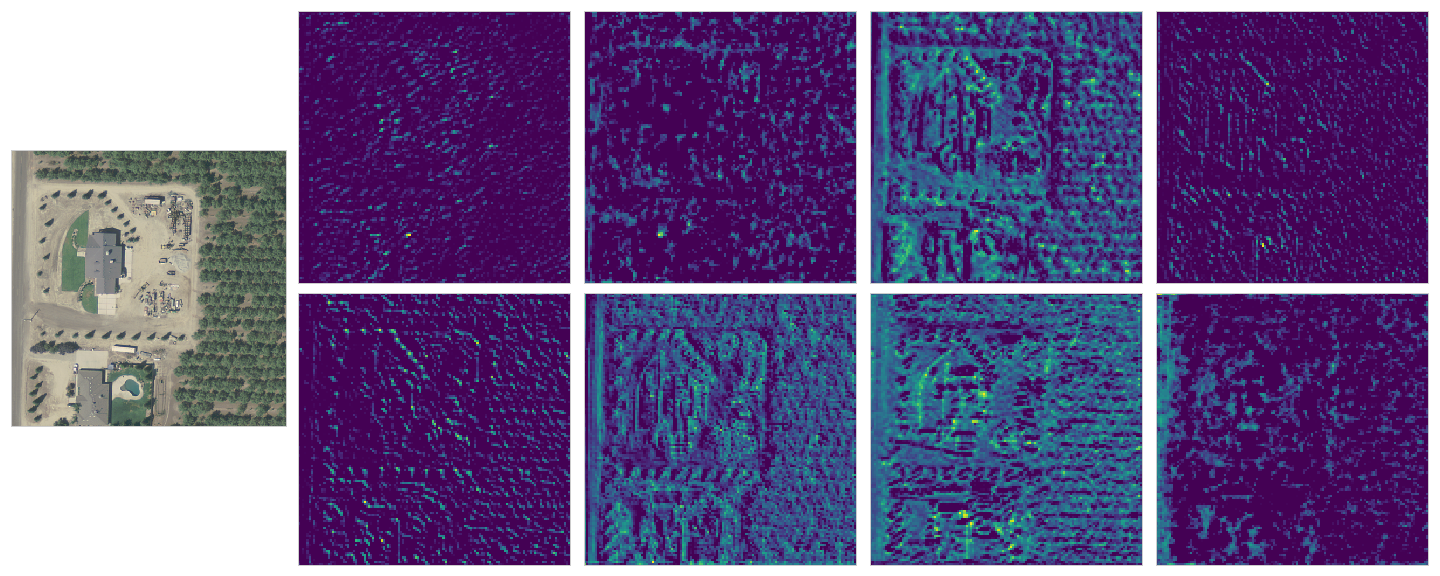
\includegraphics[width=0.9\textwidth]{Figures/activations/agriculture_l2_s1_activation_10.png}
	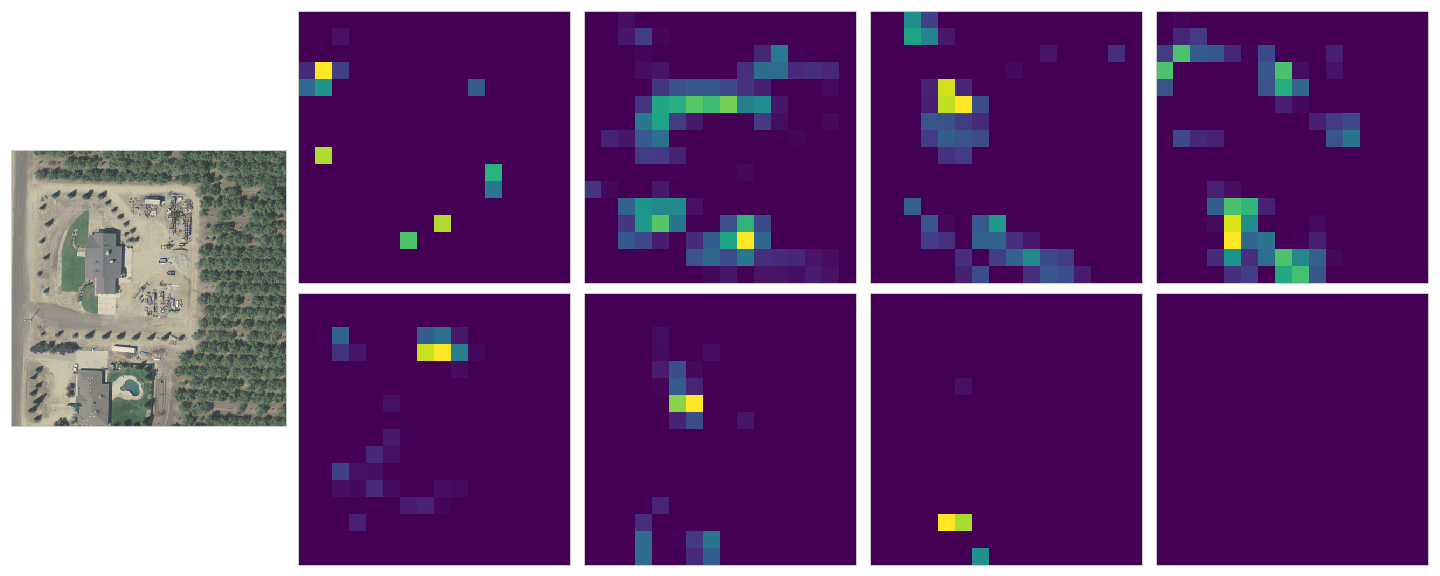
\includegraphics[width=0.9\textwidth]{Figures/activations/agriculture_l2_s1_activation_49.png}
	\captionsetup{width=1\linewidth}
	\caption{\textbf{ResNet activations of an Agriculture image: $10^{th}$ layer (top) and final layer, $49^{th}$ (bottom).}}
	\label{fig:act_agriculture}
\end{figure}

\begin{figure}[h!]
	\centering
	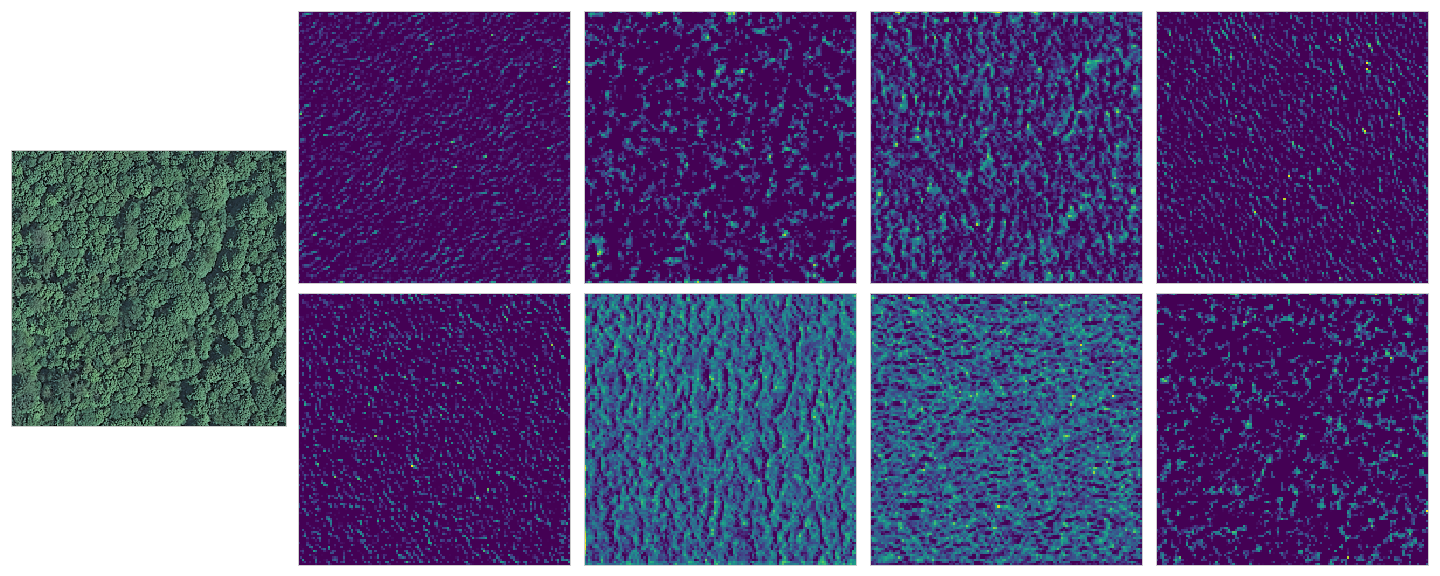
\includegraphics[width=0.9\textwidth]{Figures/activations/forest-woodland_l0_s1_activation_10.png}
	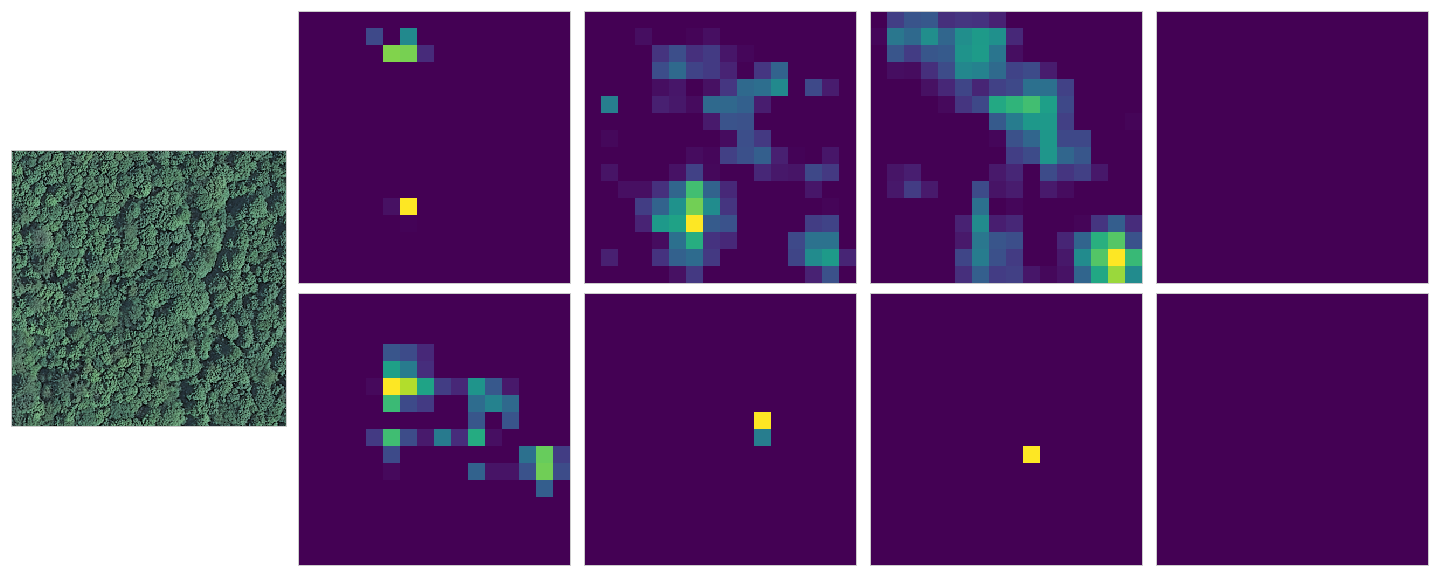
\includegraphics[width=0.9\textwidth]{Figures/activations/forest-woodland_l0_s1_activation_49.png}
	\captionsetup{width=1\linewidth}
	\caption{\textbf{ResNet activations of a Forest-woodland image: $10^{th}$ layer (top) and final layer, $49^{th}$ (bottom).}}
	\label{fig:act_forest_woodland}
\end{figure}

\begin{figure}[h!]
	\centering
	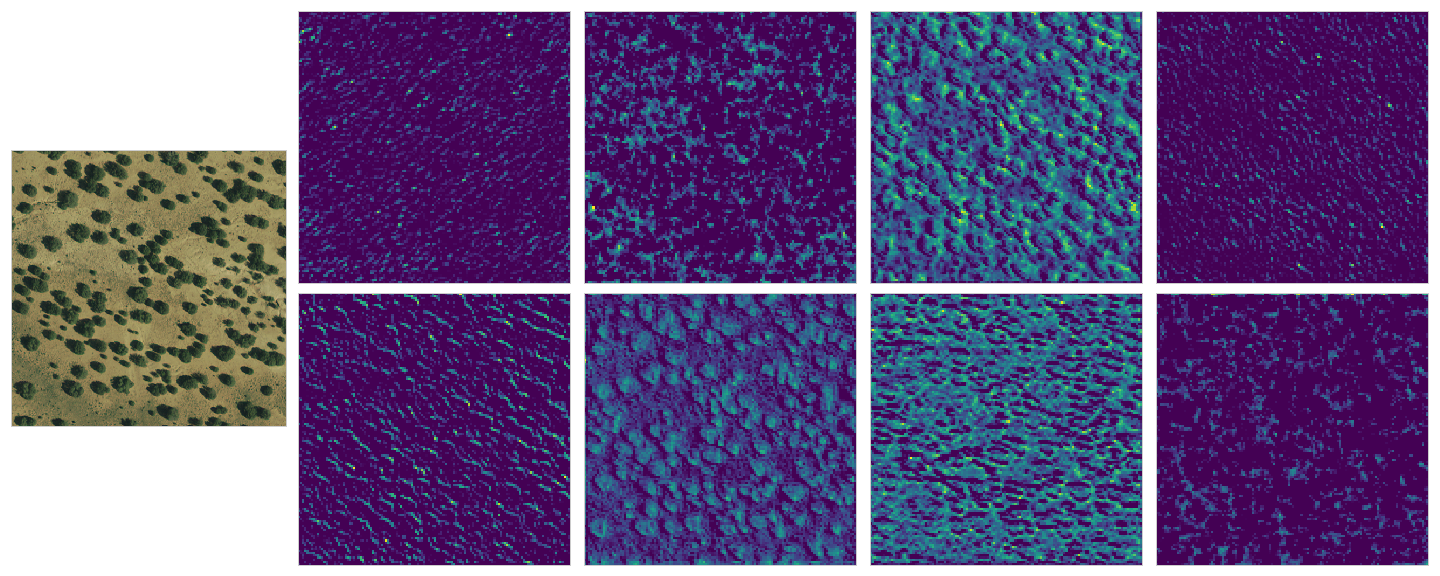
\includegraphics[width=0.9\textwidth]{Figures/activations/semi-desert_l0_s1_activation_10.png}
	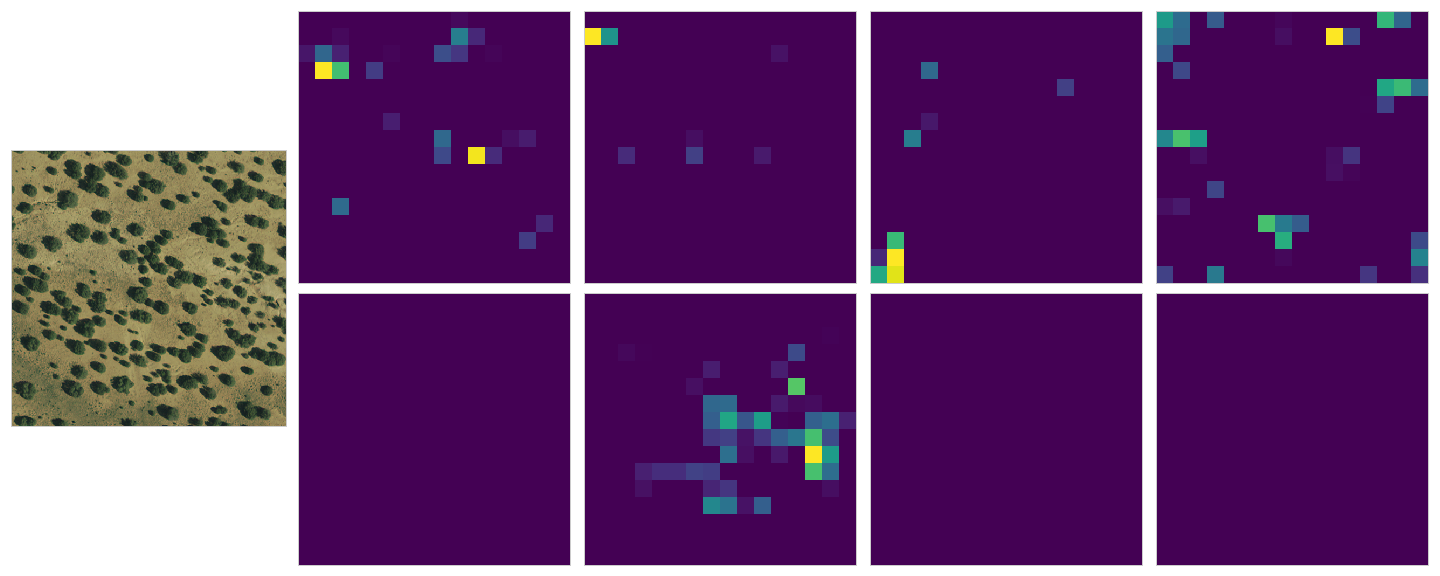
\includegraphics[width=0.9\textwidth]{Figures/activations/semi-desert_l0_s1_activation_49.png}
	\captionsetup{width=1\linewidth}
	\caption{\textbf{ResNet activations of a Semi-desert image: $10^{th}$ layer (top) and final layer, $49^{th}$ (bottom).}}
	\label{fig:act_semi_desert}
\end{figure}

\begin{figure}[h!]
	\centering
	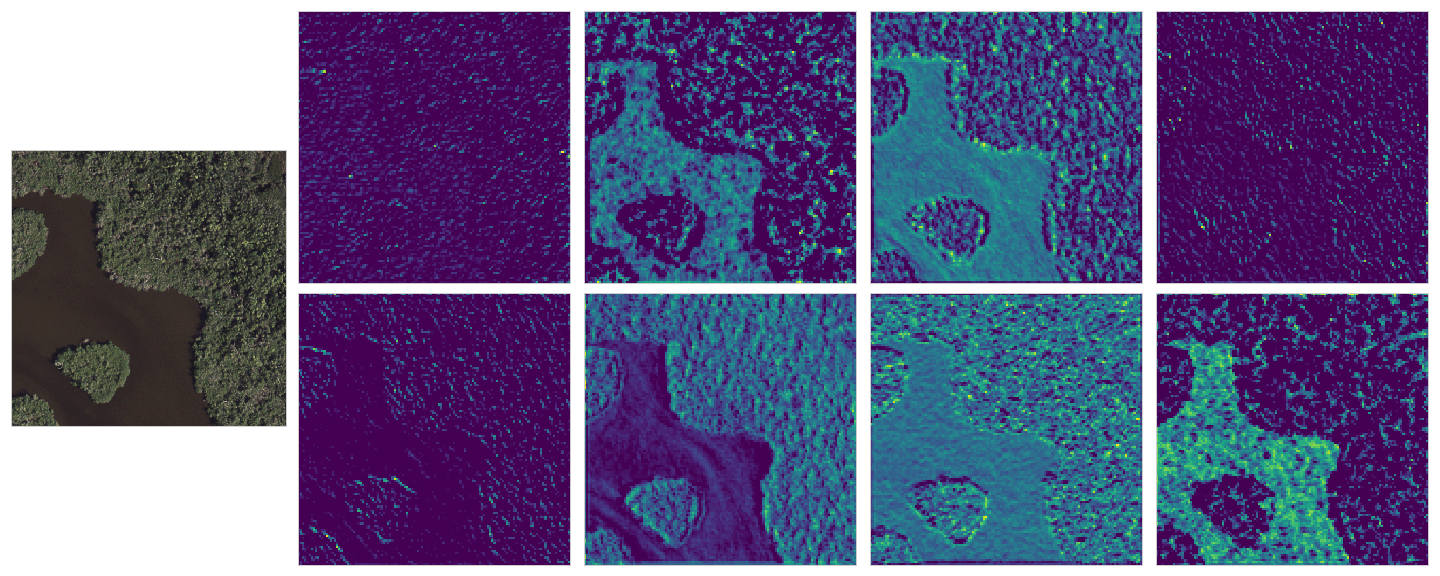
\includegraphics[width=0.9\textwidth]{Figures/activations/shrubland-grassland_l0_s1_activation_10.png}
	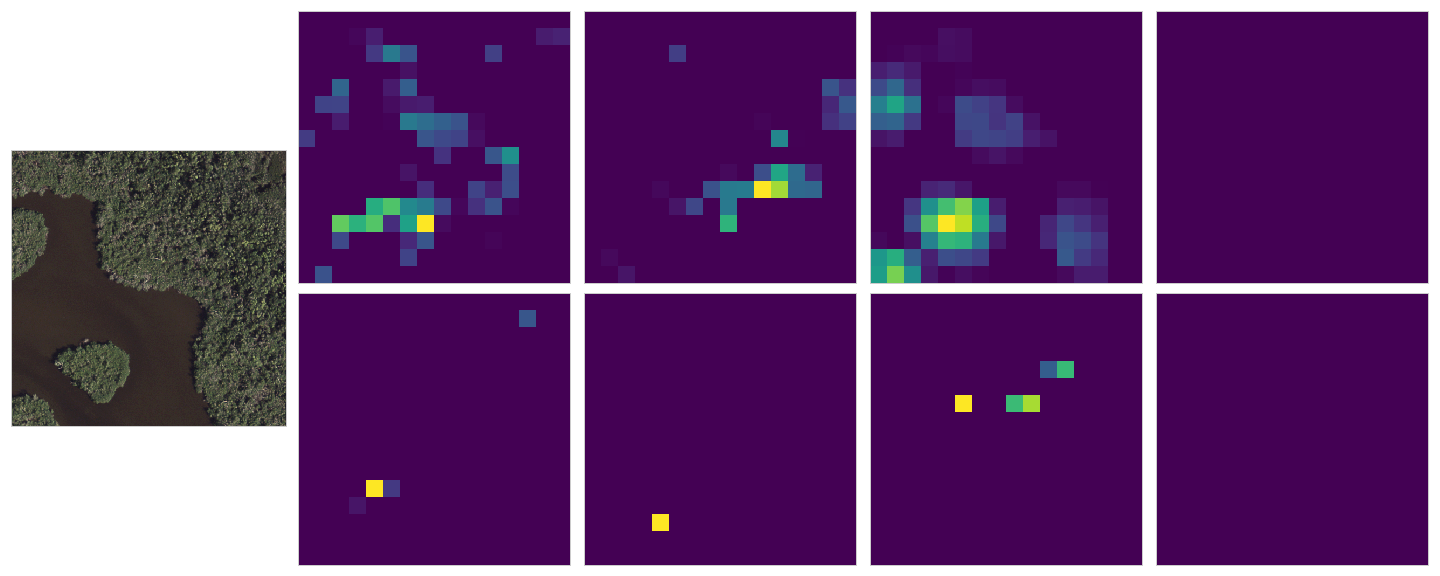
\includegraphics[width=0.9\textwidth]{Figures/activations/shrubland-grassland_l0_s1_activation_49.png}
	\captionsetup{width=1\linewidth}
	\caption{\textbf{ResNet activations of a Shrubland-grassland image: $10^{th}$ layer (top) and final layer, $49^{th}$ (bottom).}}
	\label{fig:act_shrubland_grassland}
\end{figure}


\subsection{Complete architecture}

For our purpose we considered the last ($49^{th}$) activation layer of the ResNet as the features of our images. These features can be extracted and saved on disk in order to speed up the process (as we did), or computed each time, and then passed through a simple Neural Network.

Then, our model consisted on a single dense layer of $100$ neurons with ReLU activation, followed by a single Dense node with a Sigmoid activation acting as the classifier. This model is then trained on the dataset with and RMSprop optimizer and a binary cross-entropy loss function. This same architecture is then used and trained separately for each of the resolutions considered.

\

This architecture (see Fig. \ref{fig:transfer_learning}) has been implemented with Python and Keras. Figure \ref{fig:model_keras} shows the model build, while in the following section we describe the complete training pipeline with more detail.

\begin{figure}[h!]
	\centering
	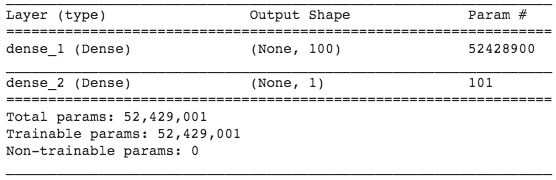
\includegraphics[width=0.7\textwidth]{Figures/model_keras.png}
	\captionsetup{width=1\linewidth}
	\caption{\textbf{Model build with Keras}}
	\label{fig:model_keras}
\end{figure}


\subsection{Training pipeline and experiments}

As introduced in previous chapters, our goal with this model is to study how feasible it is (technically and costly speaking) to detect different kind of human impact on satellite images, and how this detection behaves for different image resolutions. To do so, we build two datasets of annotated images at base resolutions of $0.3m$ and $1m$ (see Chapter \ref{Chapter2}). We then use these two datasets

In order to perform the experiments, we consider the following pipeline for each of the datasets ($0.3m$ and $1m$ resolution):

\begin{enumerate}
	\item Load the original images (at the original resolution) from disk.
	\item Downsample the images to the desired resolution.
	\item Compute the ResNet activations (at the $49^{th}$ activation layer) of the resulting images (and save to disk for later use).
	\item Consider a stratified KFold split of the dataset (with $8$ splits) for cross-validation. That means, the dataset is split into $8$ sets with labels $0-1$ equally distributed.  
	\item Train the model separately for each combination of $7$ train sets, with the remaining one as validation. Then results of the $8$ experiments are averaged for more consistency.
	\item Repeat for all downgraded resolutions needed.
\end{enumerate}

Further experiments in order to fine-tune the model complexity and the splitting parameters could be done, but it is not the goal of this project.

\begin{figure}[h!]
	\centering
	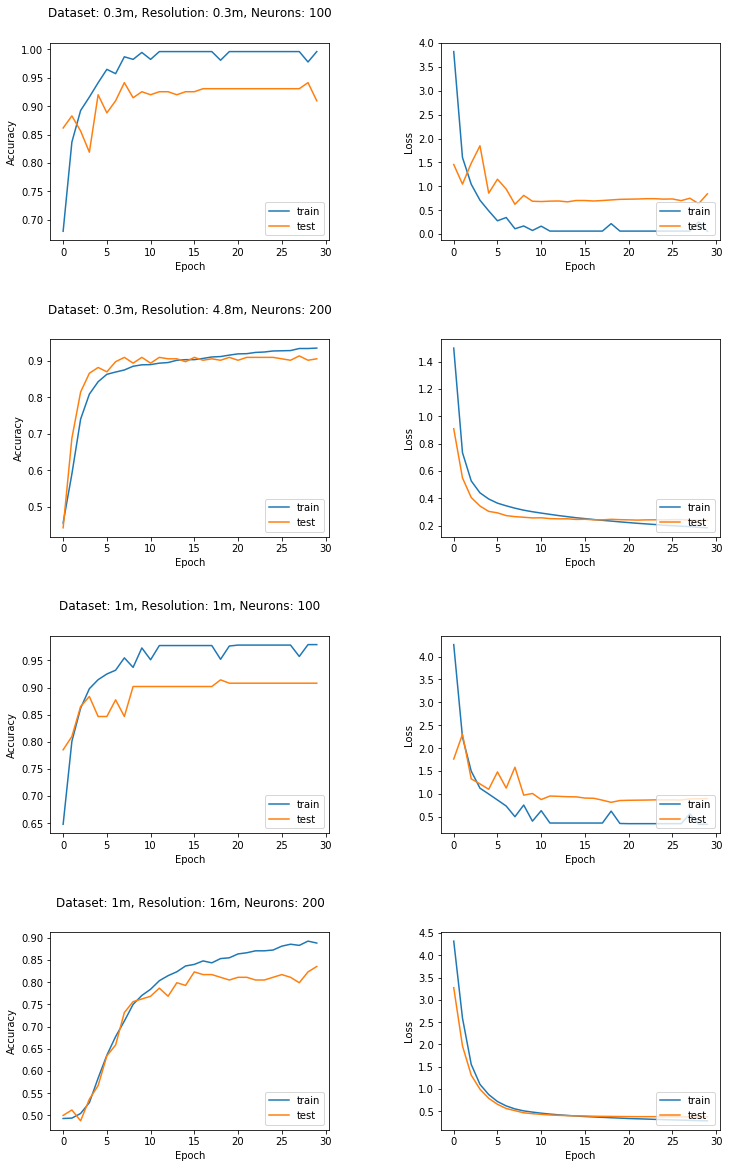
\includegraphics[width=0.9\textwidth]{Figures/results/convergence_plots_all_res.png}
	\captionsetup{width=1\linewidth}
	\caption{\textbf{Convergence plots for all downgraded resolutions of the $0.3m$ dataset.}}
	\label{fig:conv_plots}
\end{figure}

- discussion about resolutions considered, table of resolutions

\vspace{2cm}

Transfer learning: 

\begin{itemize}
	\item https://www.youtube.com/playlist?list=PLC1qU-LWwrF64f4QKQT-Vg5Wr4qEE1Zxk
	\item http://cs231n.github.io/transfer-learning/
	\item VGG: \url{https://arxiv.org/abs/1409.1556}
	\item \url{https://iopscience.iop.org/article/10.1088/1742-6596/1087/6/062032/pdf}
	\item \url{https://arxiv.org/abs/1805.02294}
	\item \url{https://cs.nyu.edu/~fergus/papers/zeilerECCV2014.pdf}
	\item \url{https://towardsdatascience.com/transfer-learning-from-pre-trained-models-f2393f124751}
	\item \url{https://www.mitpressjournals.org/doi/pdf/10.1162/neco_a_00990}
	\item \url{https://towardsdatascience.com/a-comprehensive-hands-on-guide-to-transfer-learning-with-real-world-applications-in-deep-learning-212bf3b2f27a}
\end{itemize} 

\chapter{Results} 

\label{Chapter5}

%----------------------------------------------------------------------------------------

\section{Transfer Learning on Aerial Imagery}

\section{Man-made Structures Detection at Different Scale}

\textcolor{red}{RE-DO PLOTS}

\begin{figure}[h!]
	\centering
	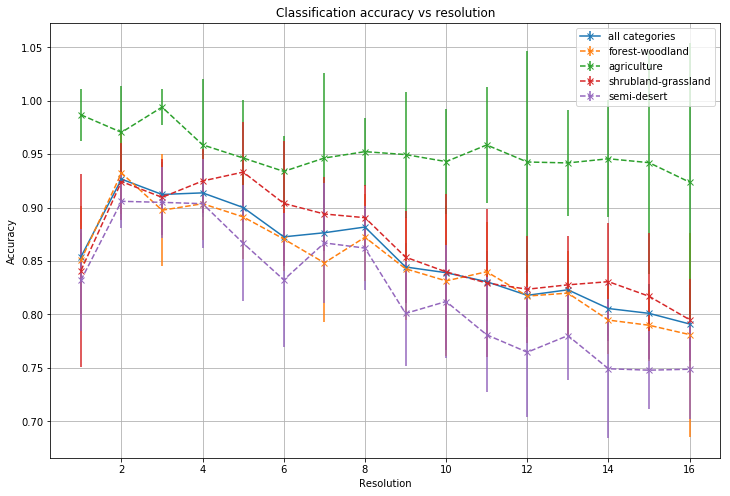
\includegraphics[width=\textwidth]{Figures/results_1m_all_categories.png}
	\captionsetup{width=1\linewidth}
	\caption{\textbf{$1m$ dataset}}
	\label{fig:acc_1m_all_cat}
\end{figure}

\begin{figure}[h!]
	\centering
	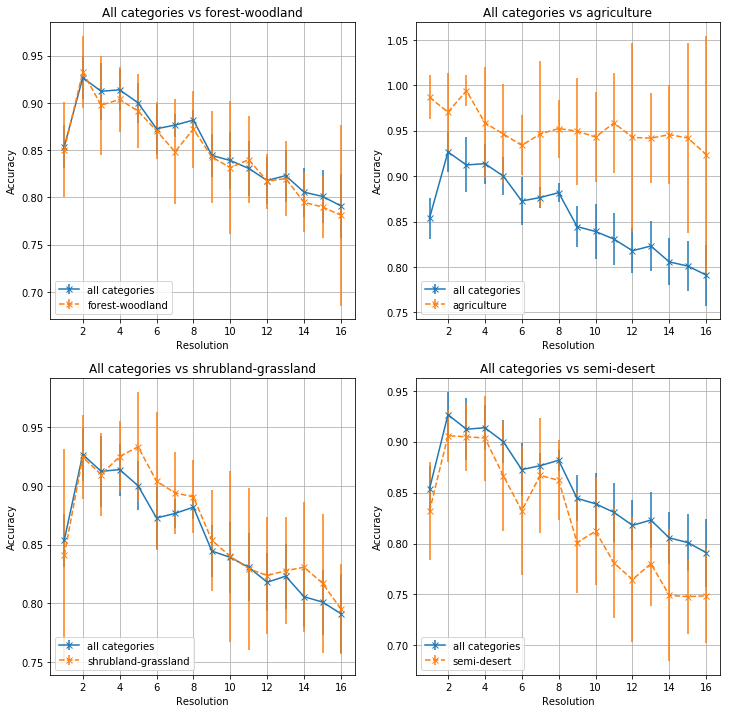
\includegraphics[width=\textwidth]{Figures/results_1m_by_category.png}
	\captionsetup{width=1\linewidth}
	\caption{\textbf{$1m$ dataset}}
	\label{fig:acc_1m_byl_cat}
\end{figure}



\section{Cost and Environment impact}


\chapter{Conclusions}

\label{Chapter6}

%----------------------------------------------------------------------------------------

\section{The Problem}

The intial phase of the project consisted on clearly defining the problem to study. The goal was to investigate which satellite imagery resolutions allowed for an accurate detection of man-made structures (or human activity), and which would be the cost associated. Hence, we needed to define the scope of human impact to consider, look for datasets suitable for this need (and eventually build our own datasets), and define the technical problem to be modeled, in order to evaluate the accuracy at each resolution. Both for the datasets and the problem, we needed them to be feasible enough to not require high technical and computational efforts, which for instance would be the case of detecting every single human activity in the images, providing their position and shape, and classifying into several categories. On the other hand, it should be a realistic enough situation, so the results obtained could be extrapolated to other, more complex scenarios.

\section{The Datasets}

As we could not find a dataset suitable for our purpose, we decided to build our own dataset. It had to be representative enough to be a challenge for our models, yet feasible to be build. Of course, having annotated images with high degree of detail, like position, shapes and types of man-made or natural structures, would be great to build high performance models.

All in all, ...

\section{The Models}

- Classification problem considered

- Feasability

- Great accuracy, decreasing for lower resolutions

\section{Further work}

\begin{itemize}
	\item Dataset: improve it, enlarge with more and more variate images, better classify them, even anotate with more categories of actual objects appearing, consider annotating areas, and train a model to detect this particular patterns. Yet, all this would diverge from the original scope of the project,
	\item Model: CNN feature extraction, other architectures and number of activations, layers, neurons, training epochs. Make a more robust pipeline, load images on batches, so a larger dataset can be considered. Implement some sort of data augmentation if needed
	\item Results: further study on which images the models fail, what kind of information is learning (patters, colors, shapes, etc)
	\item Conclusions: further analysis costs of such implementations, environment impact, etc
\end{itemize}
% Chapter 1

\chapter{Author Contributions} % Main chapter title

\label{Chapter7} % For referencing the chapter elsewhere, use \ref{Chapter1} 

%----------------------------------------------------------------------------------------

% Define some commands to keep the formatting separated from the content 
%\newcommand{\keyword}[1]{\textbf{#1}}
%\newcommand{\tabhead}[1]{\textbf{#1}}
%\newcommand{\code}[1]{\texttt{#1}}
%\newcommand{\file}[1]{\texttt{\bfseries#1}}
%\newcommand{\option}[1]{\texttt{\itshape#1}}

%----------------------------------------------------------------------------------------

This thesis is a group project between Eduard Ribas Fernández and Peter Weber. Here we will describe the individual contributions of each author. Overall, both authors have contributed to all parts in this project with different weights in each part.

In the first major block, the generation of the dataset, the distribution is as follows. The image search and download of the raw images was performed by P. Weber, while programming the image processing pipeline was done by both authors with similar weight. The labeling of the processed images was also done by both authors.

In the second major block, the data analysis pipeline, P. Weber has higher contribution at the beginning of the pipeline i.e. prototyping first solutions using transfer learning. E. Ribas has higher contribution towards the end of the pipeline. This includes optimizing the code for Colab, tuning the hyperparamters, performing analysis per category and producing the final figures.
Regarding estimation of the cost, both authors have equal contribution.

The same applies for preparing all documents related to this project (Github repository, high-level overview, thesis document), both authors have equally contributed.


%----------------------------------------------------------------------------------------
%	THESIS CONTENT - APPENDICES
%----------------------------------------------------------------------------------------

\appendix % Cue to tell LaTeX that the following "chapters" are Appendices

% Include the appendices of the thesis as separate files from the Appendices folder
% Uncomment the lines as you write the Appendices

%% Appendix A

\chapter{Frequently Asked Questions} % Main appendix title

\label{AppendixA} % For referencing this appendix elsewhere, use \ref{AppendixA}

\section{How do I change the colors of links?}

The color of links can be changed to your liking using:

{\small\verb!\hypersetup{urlcolor=red}!}, or

{\small\verb!\hypersetup{citecolor=green}!}, or

{\small\verb!\hypersetup{allcolor=blue}!}.

\noindent If you want to completely hide the links, you can use:

{\small\verb!\hypersetup{allcolors=.}!}, or even better: 

{\small\verb!\hypersetup{hidelinks}!}.

\noindent If you want to have obvious links in the PDF but not the printed text, use:

{\small\verb!\hypersetup{colorlinks=false}!}.

%\include{Appendices/AppendixB}
%\include{Appendices/AppendixC}

%----------------------------------------------------------------------------------------
%	BIBLIOGRAPHY
%----------------------------------------------------------------------------------------


\printbibliography[heading=bibintoc]


%----------------------------------------------------------------------------------------

\end{document}  
